
\section{Case Studies}

We evaluate Finch on a broad set of applications to showcase it's efficiency,
flexibility, and expressibility. All of our implementations highlight the
benefits of data structure and algorithm co-design.  Our implementation of
sparse-sparse-matrix multiply (SpGEMM) translates classical lessons from sparse
performance engineering into the language of Finch, using temporaries and
randomly-accessible workspace formats to efficiently implement the three main
approaches. Our study of sparse-matrix-dense-vector multiply (SpMV) highlights
the benefits of precise structural specialization. Our studies of image
morphology and graph applications show how Finch's programming model can express more complex
real-world kernels. Finally, we explain
how flexible operators, formats, and indexing expressions in Finch have
supported a flexible implementation of the Python Array API, supporting fused exection.

All experiments were run on a single core of a 12-core 2-socket Intel Xeon E5-2695 v2 running at
2.40GHz with 128GB of memory. Finch is implemented in Julia v1.9, targeting LLVM
through Julia. All timings are the minimum of 10,000 runs or 5s of measurement,
whichever happens first.

\subsection{Sparse-Sparse Matrix Multiply (SpGEMM)}
\begin{figure}
    \begin{minipage}{0.333\linewidth}
    \begin{minted}{julia}
    @finch begin
      C .= 0
      for j=_
        for i=_
          for k=_
            C[i, j] += AT[k, i] * B[k, j]
          end
        end
      end
      return C
    end
    \end{minted}
    \end{minipage}%
    \begin{minipage}{0.333\linewidth}
    \begin{minted}{julia}
    w = Tensor(SparseByteMap(Element(0)))
    @finch begin
      C .= 0
      for j=_
        w .= 0
        for k=_
          for i=_
            w[i] += A[i, k] * B[k, j]
          end
        end
        for i=_
          C[i, j] = w[i]
        end
      end
    end
    \end{minted}
    \end{minipage}%
    \begin{minipage}{0.333\linewidth}
    \begin{minted}{julia}
    w = Tensor(SparseHash(SparseHash(Element(0))))
    @finch begin
      w .= 0
      for k=_
        for j=_
          for i=_
            w[i, j] += A[i, k] * BT[j, k]
          end
        end
      end
      C .= 0
      for j=_, i=_
        C[i, j] = w[i, j]
      end
    end
    \end{minted}
    \end{minipage}
    \caption{Inner Products, Gustavsons, and Outer Products matrix multiply in Finch}\label{fig:spgemm_listing}
\end{figure}

Sparse Matrix-Matrix Multiplication (SpGEMM) is a fundamental operation in scientific computing and data analytics. 
We compute the $M \times N$ sparse matrix $C$ as the product of $M \times K$ and $K \times N$ sparse matrices $A$ and $B$.

There are three main approaches to SpGEMM \cite[Section 2.2]{zhang2021gamma}.
%
The inner-products algorithm takes dot products of corresponding rows and columns, while the outer-products algorithm sums the outer products of corresponding columns and rows.
%
Gustavson's algorithm sums the rows of $B$ scaled by the corresponding nonzero columns in each row of $A$.
%
Inner products is known to be asymptotically less efficient than the others, as we must do a merge operation to compute each of the $O(MN)$ entries in the output \cite{ahrens2022autoscheduling}.

Figure~\ref{fig:spgemm_listing} implements all three approaches in Finch, and Figure~\ref{fig:spgemm} compares the performance of Finch to TACO.
%
Note that these algorithms mainly differ in their loop order, but that different datastructures can be used to support the various access patterns induced.
%
Although a sparse bytemap has a dense memory footprint, we use it in our Finch implemenation of Gustavson's for the smaller $O(M)$ intermediate.
%
In our Finch implementation of outer products, we use a sparse hash table, as it is fully-sparse and randomly accessible.
%
Unfortunately, TACO does not support multidimensional sparse workspaces, only supporting outer-products with a dense output, a limitation with asymptotic consequences.
%
It's also worth mentioning that the bytemap format in TACO's Gustavson's implementation is hard-wired, whereas Finch's programming model allows us to write algorithms with explicit temporary formats and transpositions.

As depicted in Figure~\ref{fig:spgemm}, Finch achieves comparable performance with TACO on smaller matrices when we use the same datastructures, and significant improvements when we use better datastructures. Finch outperforms TACO on larger matrices, with an average speedup of 1.05. \changwan{(self)may remove this number for consistency with other exps. finch\_outer\_bytemap not explained.}

\begin{figure}
	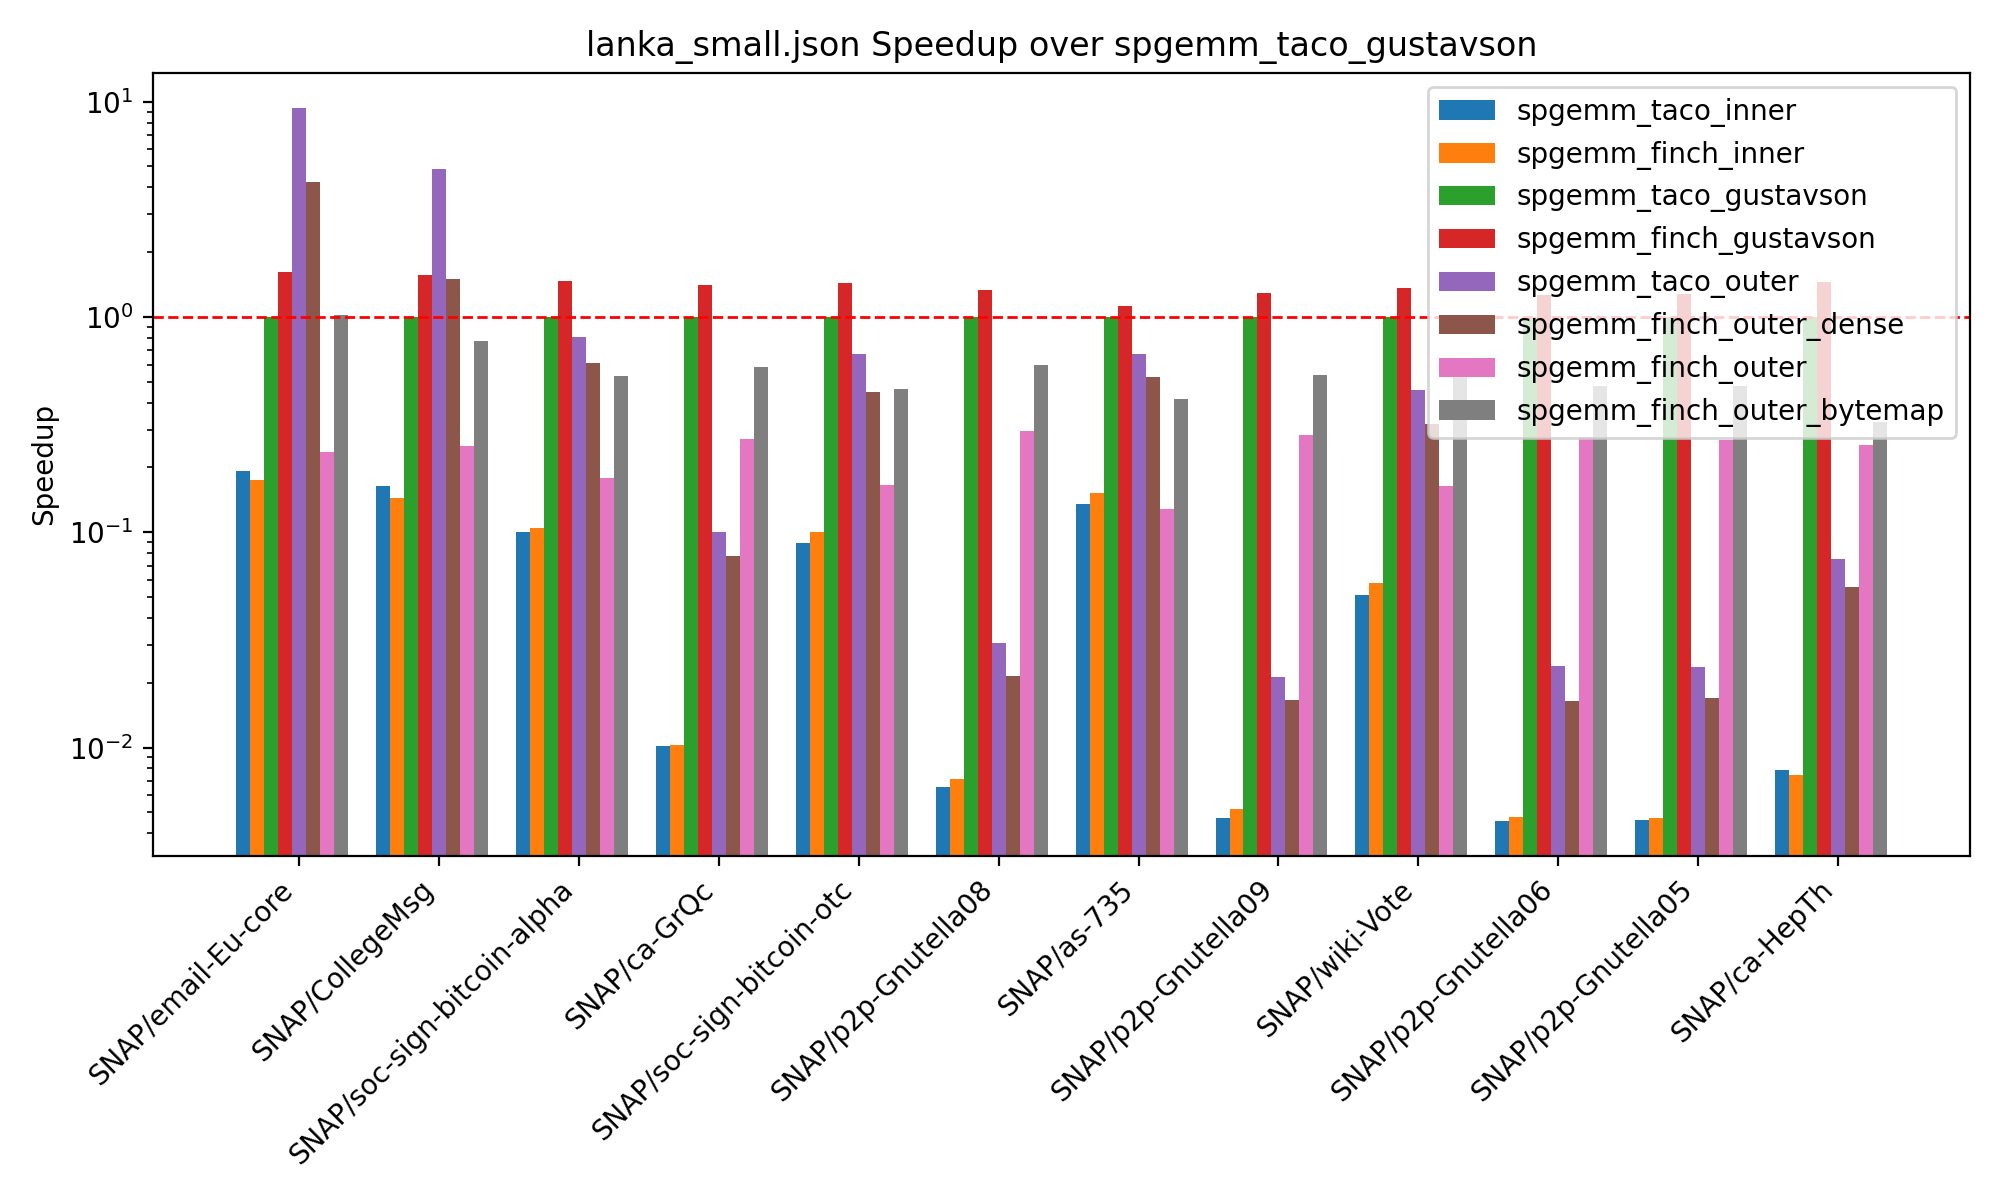
\includegraphics[width=0.5\linewidth]{spgemm_small_speedup_log_scale.png}%
	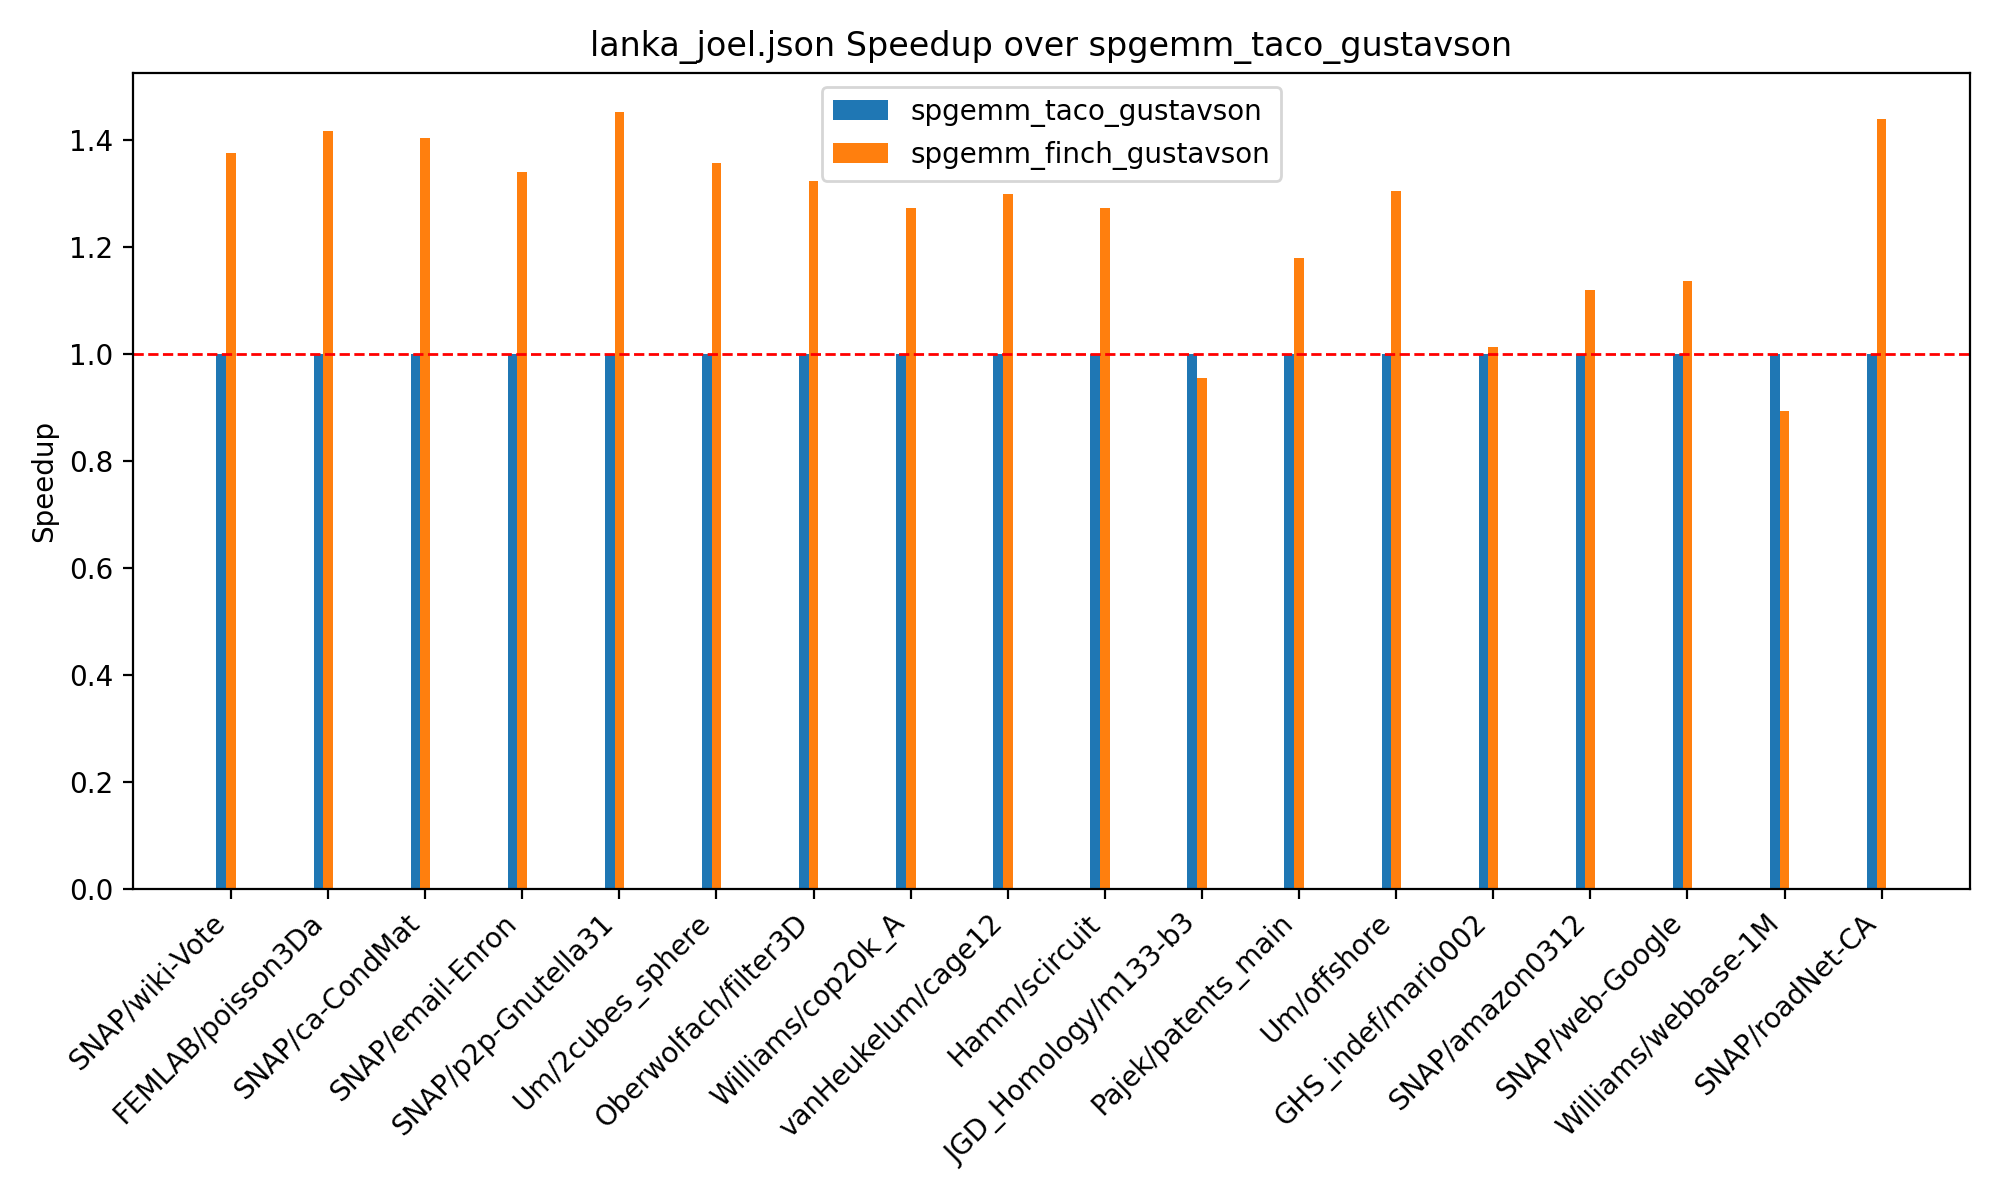
\includegraphics[width=0.5\linewidth]{spgemm_joel_speedup.png}
    \caption{A comparison of several matrix multiplication algorithms between
    Finch and Taco. On left, we use smaller matrices, ordered from small to big
    dimension. Note that inner products necessarily requires $O(n^2)$ work and
    TACO's outer products format is dense. Finch can use a sparse outer products
    format and thus has an asymptotic advantage that becomes evident as the
    output dimensions grow. On right, we use only gustavson's algorithm and
    compare on larger matrices.}
    \label{fig:spgemm}
\end{figure}

\subsection{Sparse Matrix-Vector Multiply (SpMV)}
Sparse matrix-vector multiplication (SpMV) is perhaps the most studied sparse
kernel, with a wide range of applications \cite{liu_csr5_2015,
zhou_enabling_2020}. Because SpMV is a bandwidth bound kernel, many formats have
been proposed to reduce the footprint with a minimal impact on complexity
\cite{langr_evaluation_2016}. The wide range of applications unsurprisingly
results in a wide range of structures, making it an effective kernel to
demonstrate the utility of flexible data formats. 

In this case study, we highlight different Finch formats as specified in Table \ref{spmv_tensor_formats}, and the performance effects of conforming a dataset’s structure with its storage format, which Finch's datastructure-driven model enables us to do. Finch also provides the control flow necessary to manipulate data reads and writes, enabling exploitation of multiple structural patterns concurrently (e.g. sparsity \textit{and} symmetry). 

We display speedup relative to TACO, SuiteSparseGraphBLAS, and Julia’s standard library, as depicted in Figures \ref{spmv_sorted} and \ref{spmv_grouped}.  We test using sparse matrices from a large selection of datasets spanning several previous papers: the datasets used by Vuduc et al. to test the OSKI interface \cite{vuduc2005oski}, Ahrens et al. to test a variable block row format partitioning strategy \cite{ahrens_optimal_2021}, and Kjolstad et al. to test the TACO library \cite{kjolstad_tensor_2017}. Additionally, we included the SNAP graph collection to test with boolean matrices. We also created several synthetic matrices containing bands or blocks of varying sizes as well as a permutation matrix to encapsulate a few additional use cases. The dense vector is randomly generated. We tested using the row-major and column-major Finch programs in Figure \ref{spmv_programs} as well as the symmetric program where applicable; the performance displayed for Finch on each dataset in Figure \ref{spmv_grouped} is the fastest among the formats and programs we tested. Column-major SpMV consistently performs better than row-major SpMV (an average of 1.36x better) in TACO so we use column-major SpMV in TACO as our baseline.

\begin{wrapfigure}{r}{0.41\linewidth}
    \begin{minipage}[t]{0.18\textwidth}
        \vspace{0pt} % Add this to ensure top alignment within minipage
        \begin{minted}{julia}
            y .= 0
            for j = _, i = _
              y[i] += A[i, j] * x[j]
            end
        \end{minted}
        \vspace{24pt} % Add this to ensure top alignment within minipage
        \begin{minted}{julia}
            y .= 0
            for j = _, i = _
              y[j] += A[i, j] * x[i]
            end
        \end{minted}
    \end{minipage}\hfill%
    \begin{minipage}[t]{0.22\textwidth}
        \vspace{0pt} % Add this to ensure top alignment within minipage
        \begin{minted}{julia}
            y .= 0
            for j = _
              let x_j = x[j]
                y_j .= 0
                for i = _
                  let A_ij = A[i, j]
                    y[i] += x_j * A_ij
                    y_j[] += A_ij * x[i]
                  end
                end
                #D is the diagonal
                y[j] += y_j[] + D[j] * x_j
              end
            end
        \end{minted}
    \end{minipage}
    \caption{Finch row-major, column-major and symmetric SpMV Programs}
    \label{spmv_programs}
\end{wrapfigure}



\begin{table}[htbp]
    \footnotesize
    \centering
    \caption{SpMV Tensor Formats}
    \label{spmv_tensor_formats}
    \begin{tabular}{|l|l|l|l|}
        \hline
        \textbf{Outer Level} & \textbf{Inner Level} & \textbf{Scalar Values} & \textbf{Style of Matrix}\\
        \hline
        \multirow{6}{*}{Dense} & \multirow{2}{*}{SparseList} & Element & sparse, real-valued matrices \\
        \cline{3-4} 
        & & Pattern & sparse, boolean-valued matrices \\
        \cline{2-4} 
        & SparseVBL & Element & real-valued matrices with blocked structure \\
        \cline{2-4}
        & SparseBand & Element & real-valued matrices with diagonal band \\
        \cline{2-4}
        & \multirow{2}{*}{SparsePoint} & Element & real-valued matrices with one value per row \\
        \cline{3-4} 
        & & Pattern & matrix with runs of true or false \\
        \hline 
    \end{tabular}
\end{table}

\subsubsection{Tensor Formats}
We found that the SpMV performance was superior for the level format that best paralleled the structure of the tensor. We consider the Dense(SparseList(Element)) format with the column-major SpMV program to be the Finch baseline as it is the closet analog to the sparse matrix format and SpMV program in other libraries.  

Namely, matrices with a clear blocked structure like exdata\_1, TSOPF\_RS\_b678\_c1, and heart3 performed notably well with the SparseVBL format with speedups of 2.16, 1.55, and 1.30 relative to TACO, while the baseline format had slowdowns of 0.71, 0.53, and 0.92 relative to TACO. Furthermore, the synthetic Toeplitz banded matrices we constructed performed the best with the SparseBand matrix, in particular with the toeplitz\_large\_band and the toeplitz\_medium\_band matrices having a speedup of 1.98 and 1.64 relative to TACO, while the baseline format had slowdowns of 0.84 and 0.51 relative to TACO.

There were also significant advantages of using the Pattern format instead of the Element format to represent scalar values in the matrices when these values were boolean, such as matrices in the SNAP collection which represent graph datasets are boolean. For example, the SparseList-Pattern for email-Eu-core resulted in a speedup of 2.51, while the SparseList-Element format resulted in a slowdown of 1.84 over TACO.

\begin{table}[htbp]
    \centering
    \footnotesize
    \caption{Transposed SpMV Sample Matrices}
    \label{tab:transposed_spmv_sample_matrices}
    \begin{tabular}{|
        >{\centering\arraybackslash}m{0.2\linewidth-2\tabcolsep-1.2\arrayrulewidth}|
        >{\centering\arraybackslash}m{0.2\linewidth-2\tabcolsep-1.2\arrayrulewidth}|
        >{\centering\arraybackslash}m{0.2\linewidth-2\tabcolsep-1.2\arrayrulewidth}|
        >{\centering\arraybackslash}m{0.2\linewidth-2\tabcolsep-1.2\arrayrulewidth}|
        >{\centering\arraybackslash}m{0.2\linewidth-2\tabcolsep-1.2\arrayrulewidth}|}
        \hline
         & \textbf{HB/saylr4} & \textbf{Norris/heart3} & \textbf{large\_band} & \textbf{SNAP/as-735} \\
        \hline
        \textbf{Spy} & 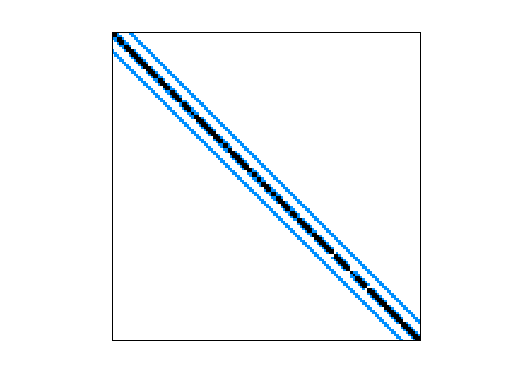
\includegraphics[width=\linewidth]{spmv_matrices/saylr4.png} & 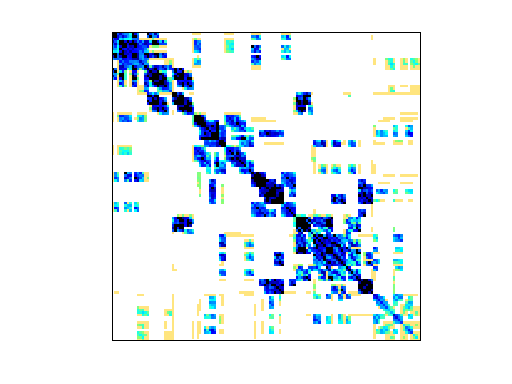
\includegraphics[width=\linewidth]{spmv_matrices/heart3.png} & 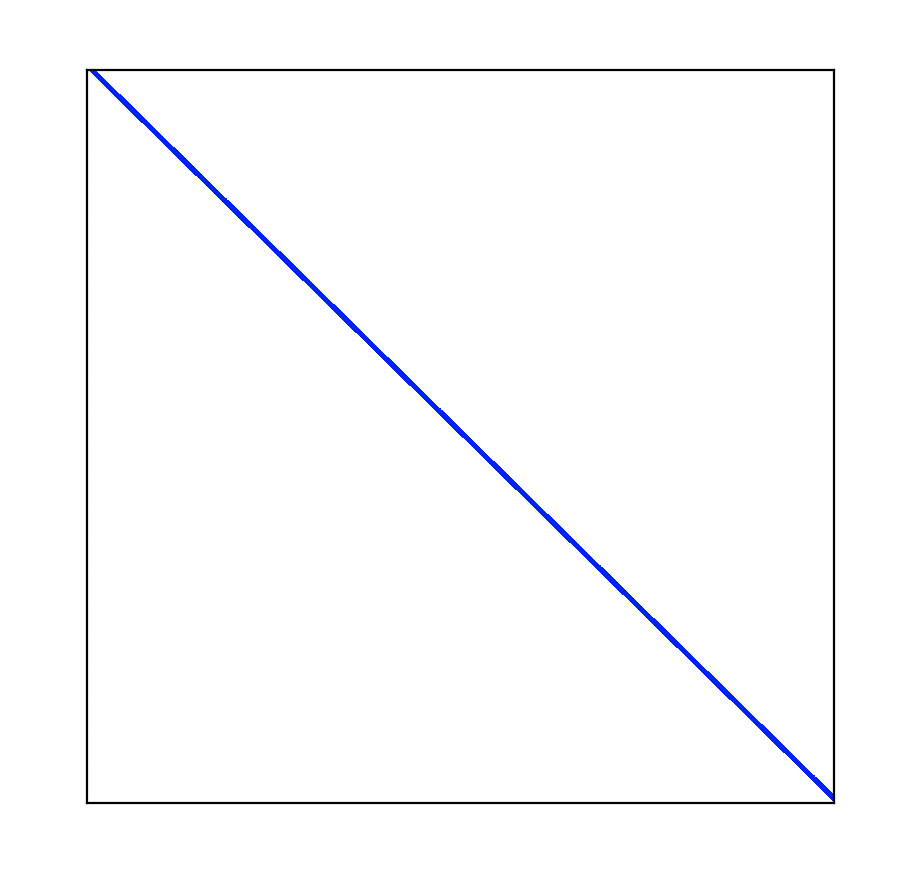
\includegraphics[width=\linewidth]{spmv_matrices/toeplitz_large_band.png} & 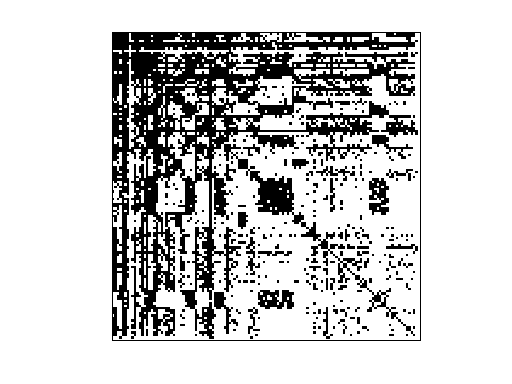
\includegraphics[width=\linewidth]{spmv_matrices/as-735.png} \\
        \hline 
        \textbf{Group / Name} & HB/saylr4 & Norris/heart3 & large\_band & SNAP/as-735 \\
        \hline
        \textbf{Dimensions} & 3,564 x 3,564 (22,316) & 2,339 x 2,339 (680,341) & 10,000 x 10,000 (1,999,900) & 7,716 x 7,716 (26,467) \\
        \hline
        \textbf{Best Finch Format} & Symmetric SparseList & SparseVBL & SparseBand & Symmetric SparseList-Pattern \\
        \hline
    \end{tabular}
\end{table}

\subsubsection{Symmetric SpMV}
Finch enables us to exploit symmetry in the sparse matrix of the SpMV kernel by providing the capabilities to reuse memory reads and insert control flow logic to restrict iterations to either the lower or upper triangle of the sparse matrix. We can apply this strategy with any level format. Every symmetric matrix in the SparseList and SparseList-Pattern formats has better performance when we use a Finch SpMV program that takes advantage of this symmetry. However, the regular row- or column-major Finch SpMV programs have better performance for symmetric matrices than the symmetric Finch SpMV program for the other more specialized formats, likely because we need in-order accesses to fully capitalize on the specialized storage. Symmetric SpMV with the SparseList level format in Finch results in an average of 1.27x speedup over TACO and symmetric SpMV with the SparseList-Pattern format in Finch results in an average speedup of 1.21x over TACO. Notably, there is a 1.91x speedup for the HB/saylr4 matrix over TACO. 

% Perhaps add the following section again in a future iteration of paper
% \subsubsection{4D Blocked SpMV}
% Finch also provides us the capability of writing an SpMV kernel [point to figure] that computes the output in blocks. Specifically, we rewrite an n x n matrix as a n/b x n/b x b x b 4-dimensional tensor and the vector as an n x n/b matrix where b is the block-size. We represent the blocked matrix with a SparseList as its second level (i.e. of format Dense(SparseList(Dense(Dense(Element(0.0)))))) so that only the non-zero blocks are stored. Then, we perform SpMV on each b x b block individually. Note that although SparseVBL already stores consecutive nonzeros in blocks, the benefit of a 4D-blocked kernel is that it additionally computes the output block by block. This method enables us to take advantage of spatial and temporal locality via register reuse [cite].

% We evaluated the 4D-blocked kernel on the Kronecker product of a neural network matrix (erdos-renyi, with sparsity p = ?) with a blocked matrix of size 10x10 and a dense and randomly generated vector. We found a 1.04x speedup to TACO, indicating comparable performance, and a 1.35x speedup to computing a non-blocked SpMV with the SparseVBL format, the fastest performing 2D Finch format for this matrix. 

% Structured matrices with induced dense blocks of equivalent size commonly arise in machine learning applications. In feature extraction, the Kronecker product of image data and a smaller matrix is computed to extract relevant features [cite]. Graph adjacency matrices or Laplacian matrices may also exhibit dense blocks when certain subsets of nodes or edges are densely interconnected. For instance, the adjacency matrix of the Erdös-Renyi random graph has a real symmetric bxb random block at each non-vanishing entry [cite]. 


%Here's a figure with spmv_performance_sorted_(faster_than_taco).png and spmv_performance_sorted_(slower_than_taco).png

\begin{figure}
    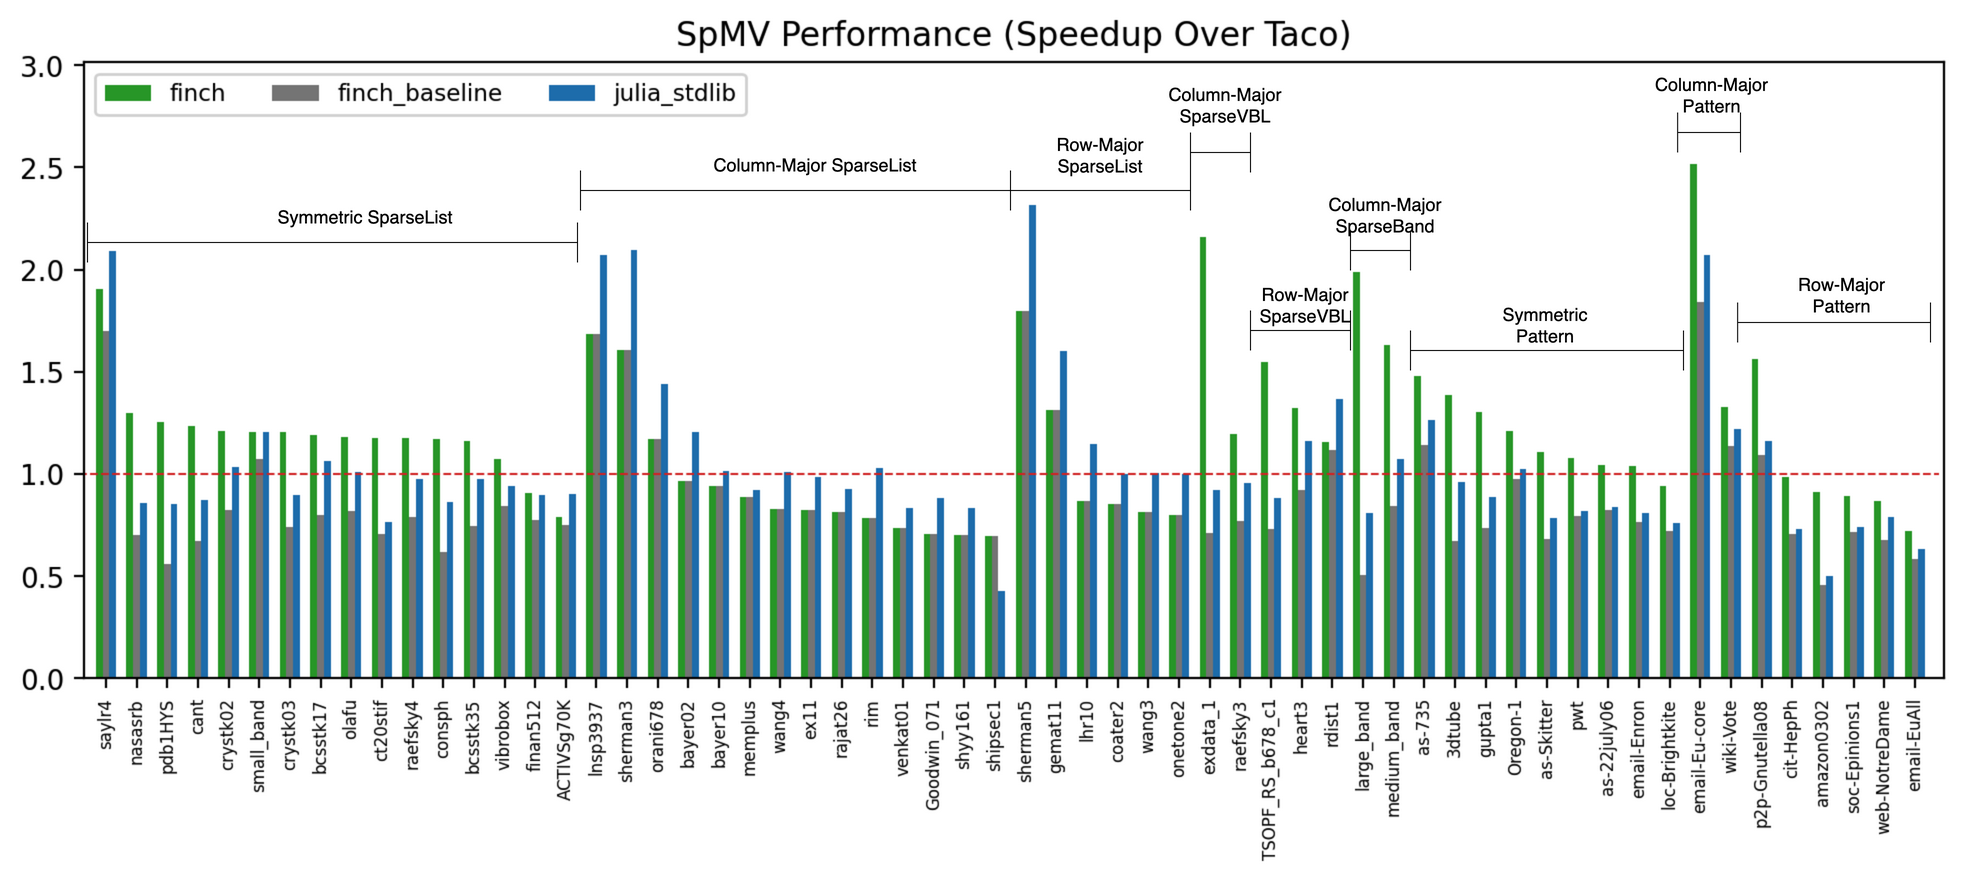
\includegraphics[width=\linewidth]{Spmv_annotated.png}
    \caption{Performance of SpMV by Finch format.}
    \label{fig:spmv_grouped}
    \footnotesize The performance displayed for Finch on each dataset is the fastest among the formats we tested. "R" indicates row-major implementation and "C" indicates column-major implementation in Finch. The baseline Finch format is unsymmetric Dense(SparseList(Element)).
\end{figure}

\subsection{Image Morphology}

Some image processing pipelines stand to benefit from structured data processing \cite{donenfeld_unified_2022}.
In this case study, we focus on binary image morpology and the logical transformation of binary images and masks.
We consider two operations: binary erosion (computing a mask), and a masked histogram (using a mask to avoid work).

Samples from our datasets are shown in Figure~\ref{fig:image_datasets}. Note that these images are all binary, either by design or having been thresholded.

Finch allows us to modify both our algorithm and our datastructure, so we may choose to use either a dense representation with bytes ($Dense(Element(0x00))$), a bit-packed representation ($Dense(Element(UInt64))$), or a run-length encoded representation that represents runs of true or false ($SparseRLE(Pattern())$).
%
All of these have their advantages.
%
The dense representation induces the least overhead, the bit-packed representation can take advantage of bitwise binary ops, and the run-length encoded version only uses memory and compute when the pattern changes between true and false.

The erosion operation turns off a pixel unless all of it's neighbors are on.
%
This can be used to shrink the boundaries of a mask, and remove point instances of noise \cite{fisher_hypermedia_1996}.
\help{link a few cool images that show erosion}
%
Note that three instances of structured data are used here, both in the mask, in the padding of the inputs, and in the convolutional filter itself.
%
We might understand the filter as a structured tensor of circular shifts, or we might understand each shifted view of the data in an unrolled stencil computation as a structured tensor.
Figure \ref{fig:erosion_listing} displays example erosion algorithms for bitwise
or run-length-encoded algorithms, and a masked histogram kernel.

We compare to OpenCV, and chose the histogram since the OpenCV histogram function also accepts a mask. If we use $SparseRLE(Pattern())$ for our mask, we can reduce the branching
in the masked kernel and get better performance.
%
We this is also an instance where we use a computed index into the output, something not many sparse and structured programming frameworks support.

We used four datasets. We randomly selected 100 images from the MNIST \cite{lecun_gradient-based_1998} and Omniglot \cite{lake_human-level_2015} character recognition datasets, as well as a dataset of human line drawings \cite{eitz_how_2012}. We also hand-selected a subset of mask images (these images were less homogenous, so we listed them in the appendix) from a digital image processing textbook \cite{gonzalez_digital_2006}. All images were thresholded, and we also include versions of the images that have been magnified before thresholding, to induce larger constant regions. IN our erosion task, the sparseRLE format performs the best as it is asymptotically faster and uses less memory, leading to a 19.5X speedup over OpenCV on the sketches dataset, which becomes arbitrarily large as we magnify the images (here shown as 266X). The improvements with SparseRLE are seen in the histogram task as well, as it allows us to
mask off contiguous regions of computation, instead of individual pixels, reducing the branches in the mask and leading to a significant speedup (20.3x on Omniglot and 20.8x on sketches. We believe the 51.6x on MNIST is due to calling overhead in OpenCV). The bitwise kernels were effective as well, and would be more effective on datasets with less structure. A strength of Finch is that it supports structured datasets, even over bitwise operations, allowing us to implement the bitwise kernel and then mask it.

\begin{figure}
    \scriptsize
    \begin{minipage}{0.5\linewidth}
    Wordwise Erosion:
    \begin{minted}{julia}
        output .= false
        for y = _
          tmp .= false
          for x = _
            tmp[x] = coalesce(input[x, ~(y-1)], true) & input[x, y] & coalesce(input[x, ~(y+1)], true)
          end
          for x = _
            output[x, y] = coalesce(tmp[~(x-1)], true) & tmp[x] & coalesce(tmp[~(x+1)], true)
          end
        end
    \end{minted}
    \vspace{12pt}
    Masked Histogram:
    \begin{minted}{julia}
        bins .= 0 
        for x=_
          for y=_
            if mask[y, x]
              bins[div(img[y, x], 16) + 1] += 1
            end
          end
        end
    \end{minted}
    \end{minipage}%
    \begin{minipage}{0.5\linewidth}
    Bitwise Erosion:
    \begin{minted}{julia}
        output .= 0
        for y = _
          tmp .= 0
          for x = _
            if mask[x, y]
              tmp[x] = coalesce(input[x, ~(y-1)], 0xFFFFFFFF) & input[x, y] & coalesce(input[x, ~(y+1)], 0xFFFFFFFF)
            end
          end
          for x = _
            if mask[x, y]
              let tl = coalesce(tmp[~(x-1)], 0xFFFFFFFF), t = tmp[x], tr = coalesce(tmp[~(x+1)], 0xFFFFFFFF)
                let res = ((tr << (8 * sizeof(UInt) - 1)) | (t >> 1)) & t & ((t << 1) | (tl >> (8 * sizeof(UInt) - 1)))
                  output[x, y] = res
                end
              end
            end
          end
        end
    \end{minted}
    \end{minipage}
    \caption{Two approaches to erosion in Finch. The $coalesce$ function defines the out of bounds value. On left, the naive approach. On $SparseRLE(Pattern())$ inputs, this only performs operations at the boundaries of constant regions. On right, a bitwise approach, using a mask to limit work to nonzero blocks of bits.}
    \label{fig:morphology_listing}
\end{figure}

\begin{figure}
	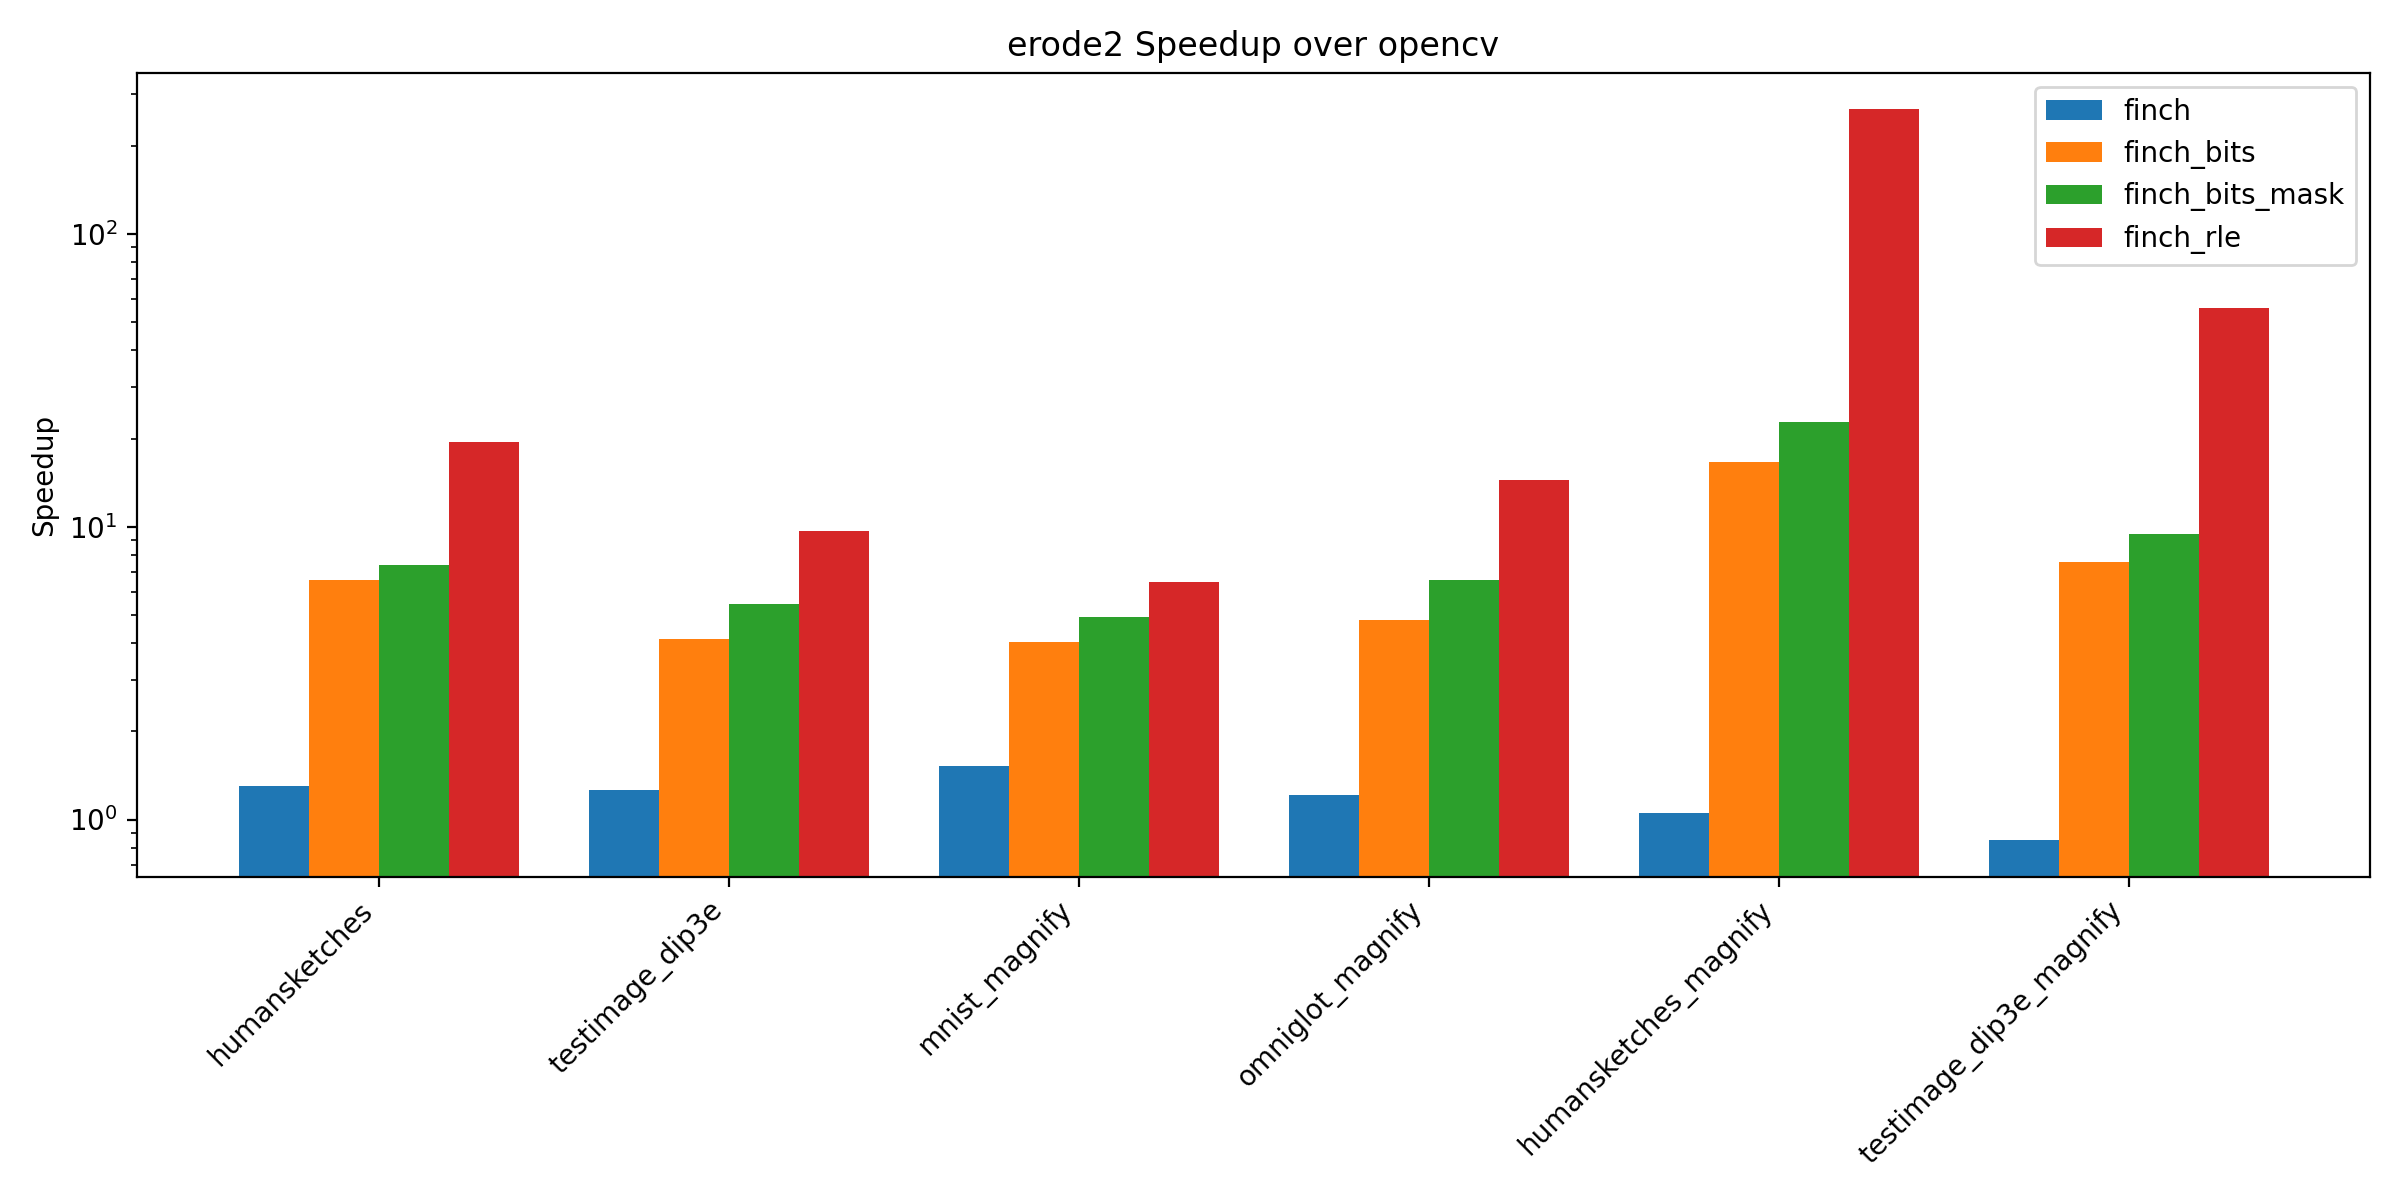
\includegraphics[width=0.5\linewidth]{erode2_speedup_over_opencv.png}%
	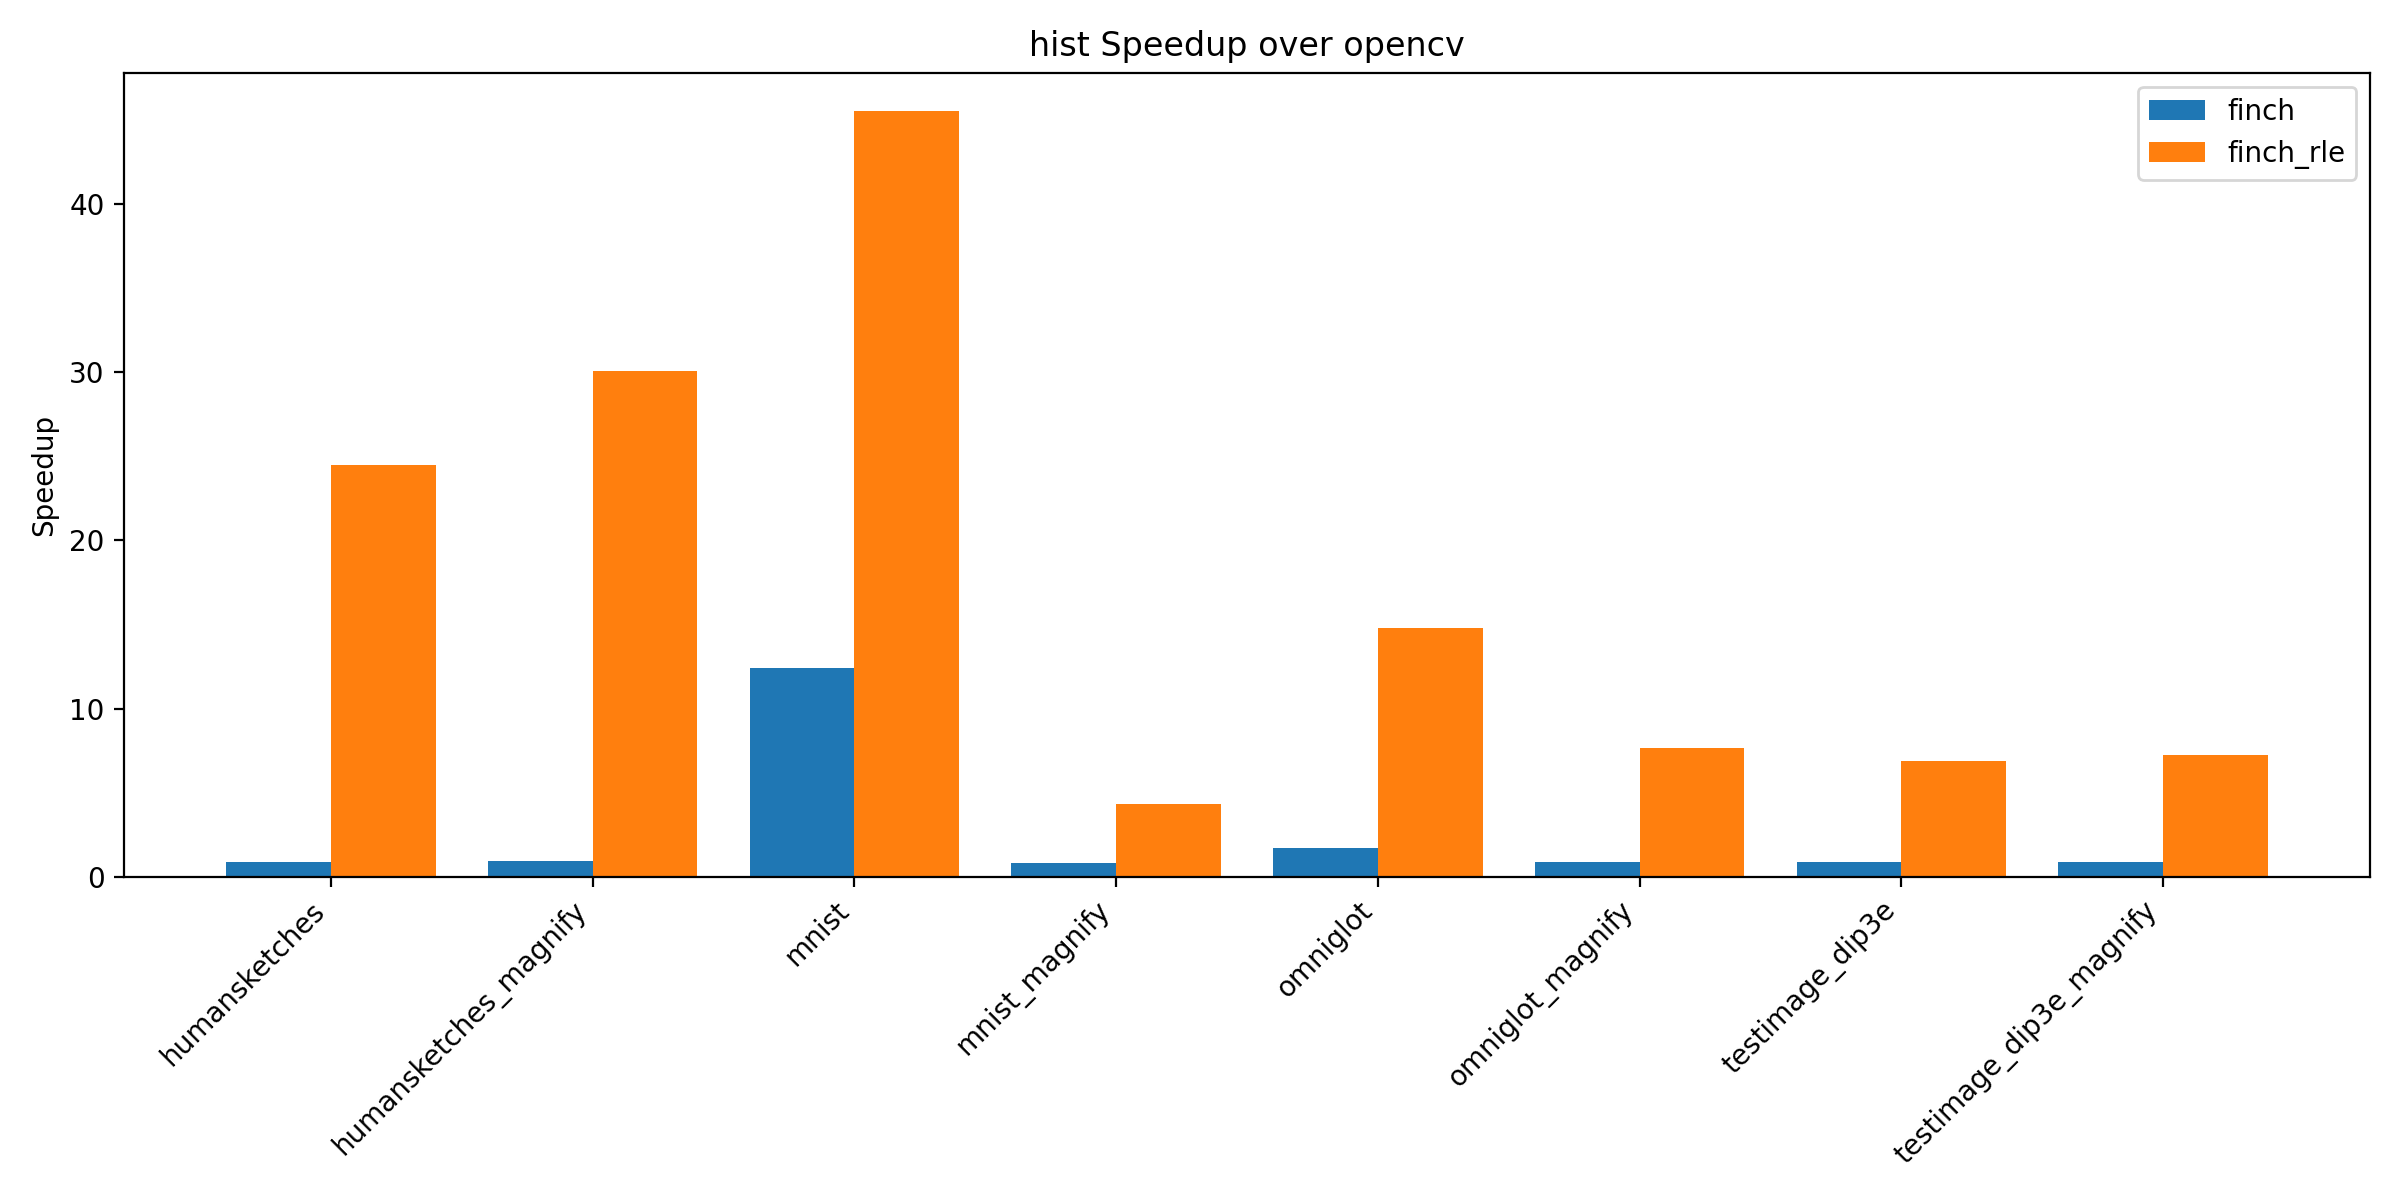
\includegraphics[width=0.5\linewidth]{hist_speedup_over_opencv.png}
    \caption{Performance of Finch on image morphology tasks. On left, we run 2 iterations of erosion. On right, we run a masked histogram.}\label{fig:morphology}
\end{figure}

\subsection{Graph Analytics}
%\help{In this case, the two main highlights are that Finch can do arbitrary operators (i.e. choose), and that Finch can do early break, and also the different loop orders and multiple outputs. We may need to explain a little bit about what push pull is. For bellman, the main point is that we need multiple outputs, sparse inputs, masks, and sparse outputs with differing formats at differing points.}

We used finch to implement two fundamental graph algorithms: Breadth-First Search (BFS) and Bellman-Ford single-source shortest path. Our BFS implementation and graphs datasets are taken from Yang et. al \cite{yang_implementing_2018}, including road networks, characterized by bounded node degrees and long diameters, and scale-free graphs, where node degree distribution follows a power-law distribution and diameters are short.

Direction-optimization~\cite{beamer2012direction} is crucial for achieving high BFS performance in such scenarios, switching between push and pull traversals to efficiently explore graphs. Push traversal visits the neighbors of each frontier node, while pull traversal visits every node and checks to see if it has a neighbor in the frontier. The advantage of pull traversal is that we may terminate our search once we find a node in the frontier, saving time in the event the push traversal were to visit most of the graph anyway. Early break is the critical part of control flow in this algorithm, though the algorithms also require different loop orders, multiple outputs, and custom operators.

Figure \ref{fig:graph_result} compares performance to Graphs.jl, an open-source Julia library, and the LAGraph Library, which implements graph algorithms in the language of linear algebra using GraphBLAS\cite{mattson2019lagraph}. For the BFS algorithm, direction-optimization notably enhances performance for scale-free graphs. Although GraphBLAS uses hardwired optimizations, Finch is competitive on these benchmarks. On Bellman-Ford (with path lengths and shortest-path tree), Finch's support for multiple outputs, sparse inputs, and masks leads to superior performance over GraphBLAS (average speedup of 1.05). Note that we did not include GAP-road as it took too long to run.
 
\begin{figure}
	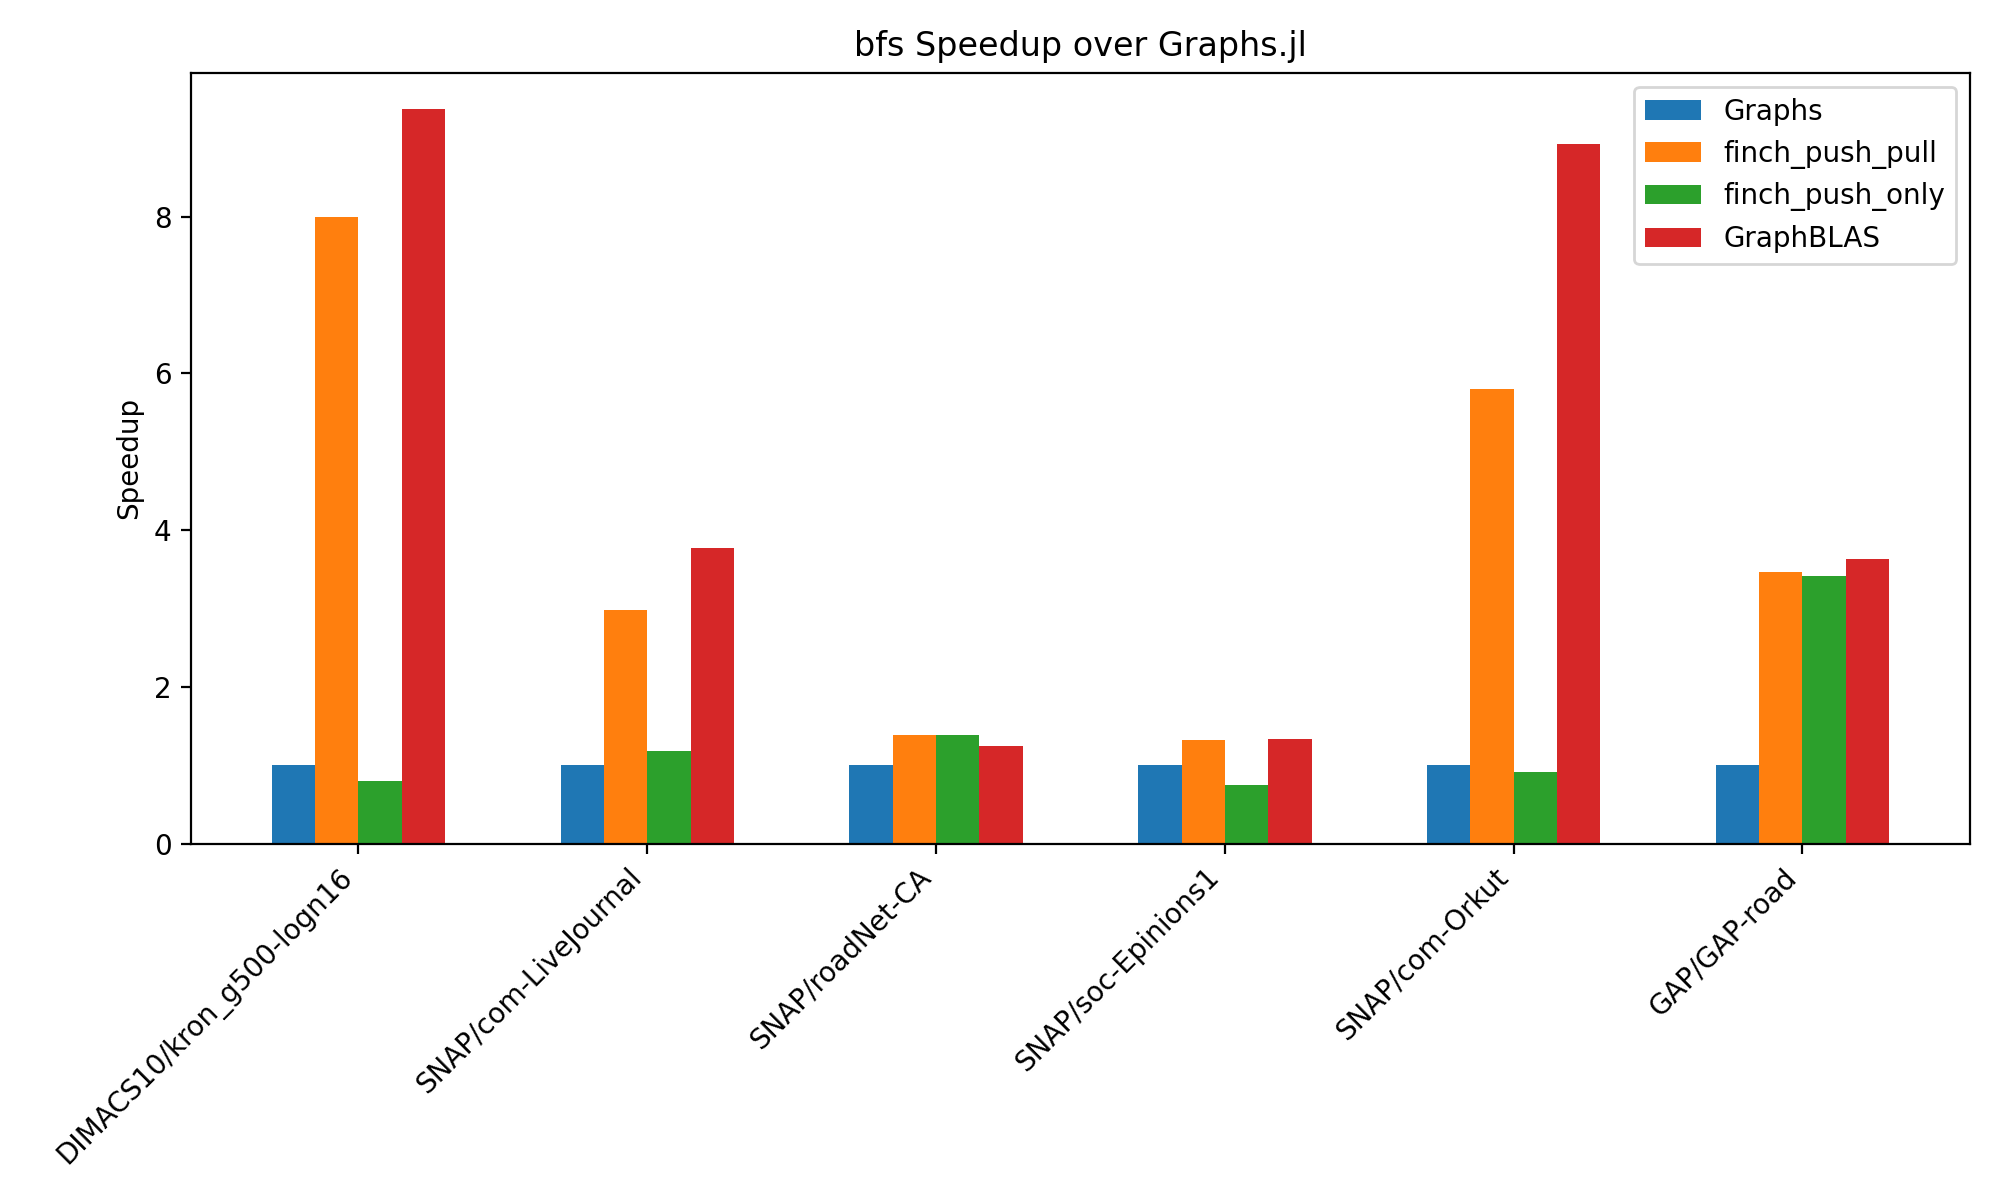
\includegraphics[width=0.5\linewidth]{bfs_speedup_over_graphs.jl.png}%
	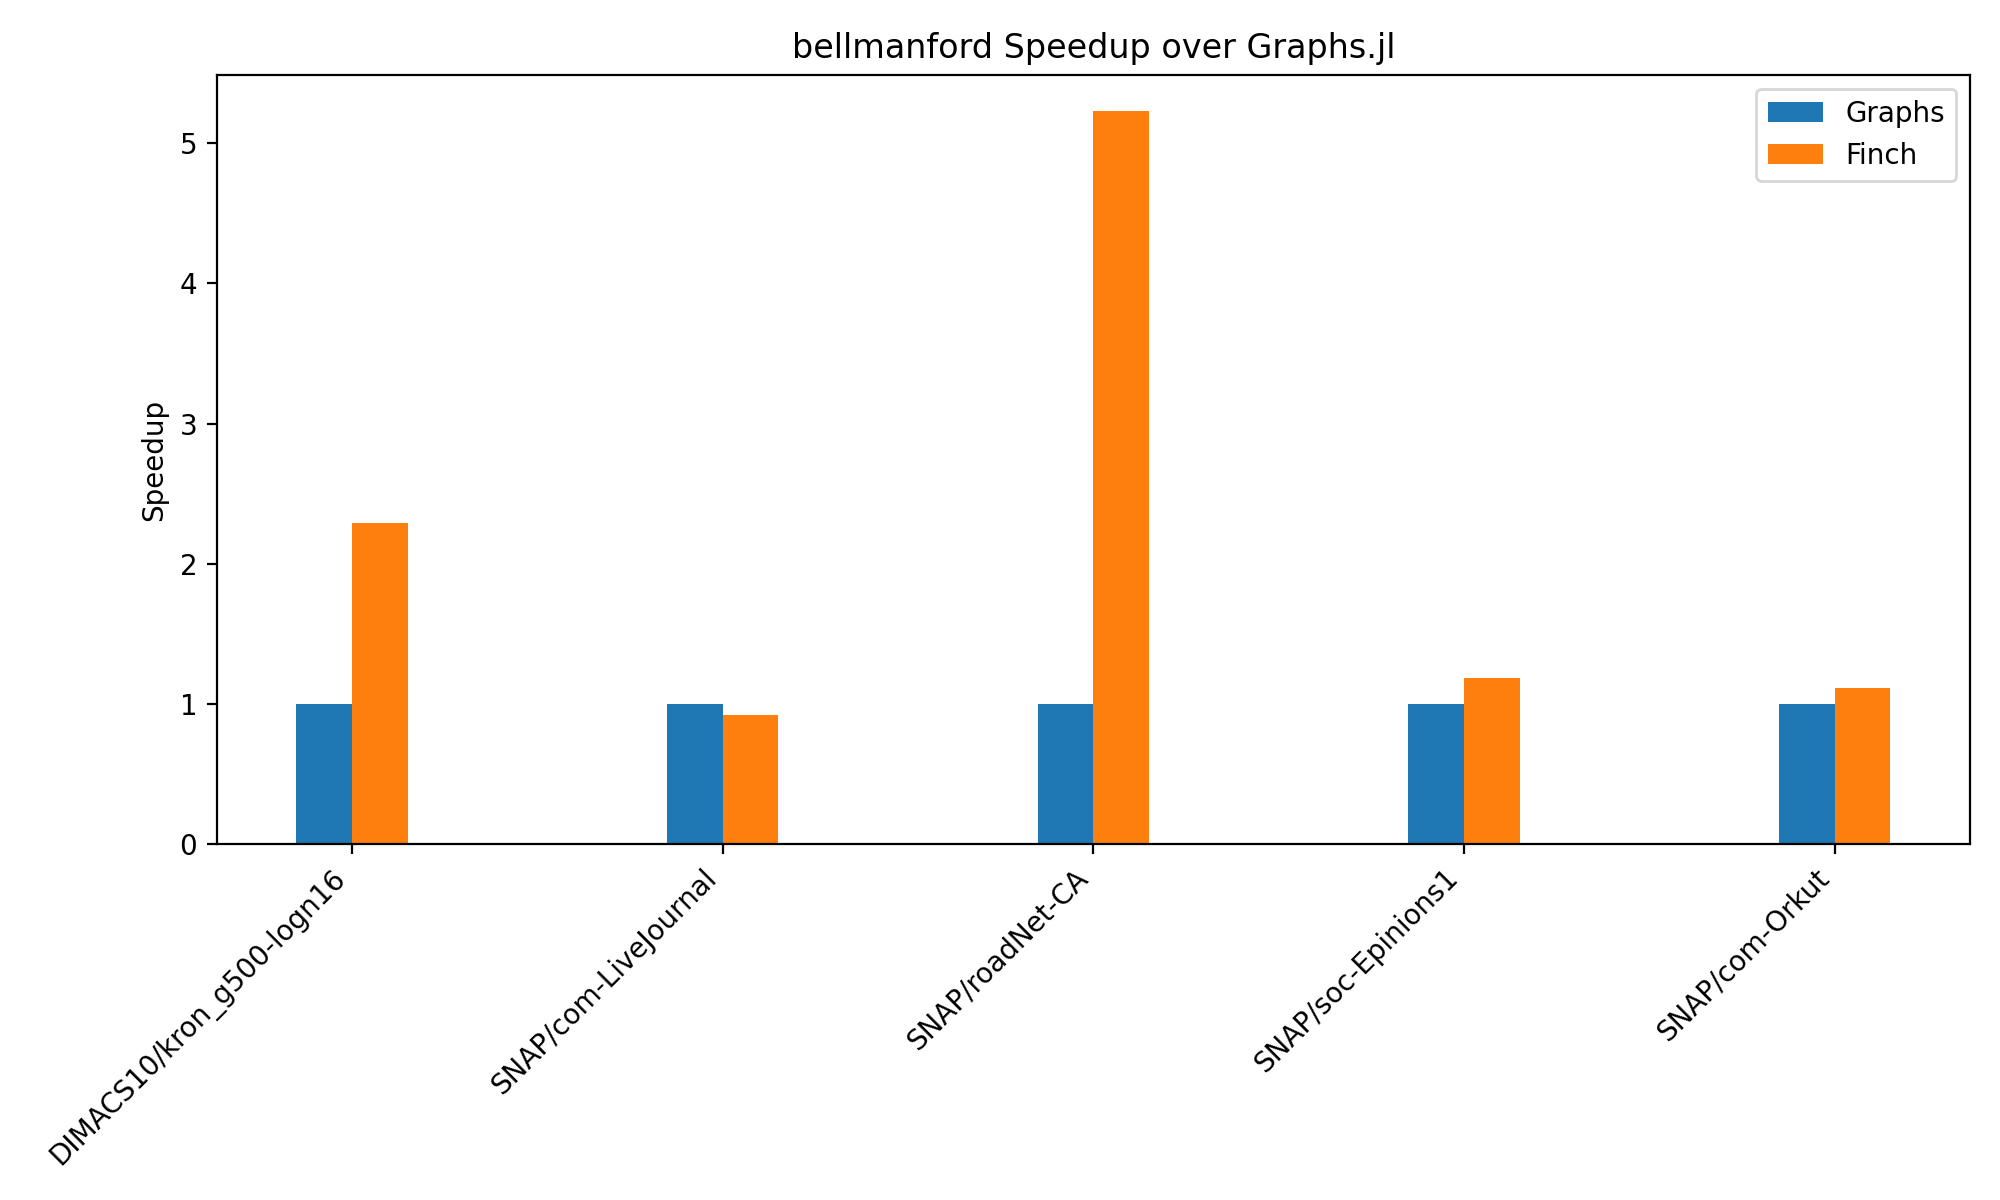
\includegraphics[width=0.5\linewidth]{bellmanford_speedup_over_graphs.jl.png}
    \caption{Performance of graph apps across various tools. finch\_push\_only exclusively utilizes push traversal, while finch\_push\_pull applies direction-optimization akin to GraphBLAS. Finch's support for push/pull traversal and early break facilitates direction-optimization. Among GraphBLAS's five variants for Bellman-Ford, we selected LAGraph\_BF\_full1a, consistently the fastest with our graphs.}
     \label{fig:graph_result}
\end{figure}

\begin{figure}
    \begin{minipage}{0.33\linewidth}
    \begin{minted}{julia}
    V = Tensor(Dense(Element(false)))
    P = Tensor(Dense(Element(0)))
    F = Tensor(SparseByteMap(Pattern()))
    _F = Tensor(SparseByteMap(Pattern()))
    A = Tensor(Dense(SparseList(Pattern())))
    AT = Tensor(Dense(SparseList(Pattern())))

    function bfs_push(_F, F, A, V, P)
      @finch begin
        _F .= false
        for j=_, k=_
          if F[j] && A[k, j] && !(V[k])
            _F[k] |= true
            P[k] <<choose(0)>>= j
          end
        end
        return _F
      end
    end

    \end{minted}
\end{minipage}%
\begin{minipage}{0.33\linewidth}
    \begin{minted}{julia}
    function bfs_pull(_F, F, AT, V, P)
      p = ShortCircuitScalar{0}()
      @finch begin
        _F .= false
        for k=_
          if !V[k]
            p .= 0
            for j=_
              if F[follow(j)] && AT[j, k]
                p[] <<choose(0)>>= j
              end
            end
            if p[] != 0
              _F[k] |= true
              P[k] = p[]
            end
          end
        end
        return _F
      end
    end
    \end{minted}
\end{minipage}%
\begin{minipage}{0.33\linewidth}
  \begin{minted}{julia}
  _D = Tensor(Dense(Element(Inf)), n)
  D = Tensor(Dense(Element(Inf)), n)
  function bellmanford(A, _D, D, _F, F)
    @finch begin
    F .= false
    for j = _
      if _F[j]
        for i = _
          let d = _D[j] + A[i, j]
            D[i] <<min>>= d
            F[i] |= d < _D[i]
          end
        end
      end
    end
  end
\end{minted}
\end{minipage}
\caption{Graph Applications written in Finch. Note that parents are calculated separately for Bellman-Ford. The $choose(z)$ operator is a GraphBLAS concept which returns any argument that is not $z$.}\label{fig:graph_listing}
\end{figure}

\subsection{Implementing Numpy's Array API in Finch}
In the past decade, the adoption of the Python Array API \cite{harris_array_2020} has allowed for a proliferation array programming systems, but existing implementations of this API for structured data suffer from either incompleteness or inefficiency. They generally either limit the dimensionality to vectors and matrices or only support tabular representations in order to reduce the complexity of interactions between different formats. Further, existing work doesn't support the fusion of arbitrary operators which can have a drastic impact on performance as we show in Fig. (\kyle{PUT FIG HERE}). We believe that a flexible, online compiler like Finch which can manage the complexity of arbitrary operations between inputs with a wide variety of formats is the secret ingredient needed to make the array API performant for structured data.

There is a gap between the expressiveness of the purely declarative Array API and the Finch language which defines both the output and the algorithm. The naive approach to solving this would be to explicitly define a mapping from each function in the API to a Finch program which eagerly produces the output. This approach results in a simple translation procedure but misses crucial opportunities for optimization across a chain of function calls and needlessly materializes large intermediate results. To avoid this, we have implemented a lazy evaluation approach that collects API calls and then computes output when requested by the user. This is implemented through 1) Finch Logic, a minimal, high-level language for expressing array operations and 2) the Finch Interpreter, which lowers Finch Logic programs to one or more Finch programs while making heuristic decisions about output format, loop ordering, and protocols.

\subsubsection{Finch Logic}
The expression fragment of the logical language takes inspiration from relational algebra while incorporating an ordering on the dimensions of a tensor. This means that every operator (with the exception of $\finchtable$ and $\finchalias$ which are analogous to the scan operator in RA) takes in an indexed tensor and outputs an indexed tensor. Conceptually, an indexed tensor can be thought of as a relation with an ordering on the index attributes and a separate value attribute, and we include the $\finchreorder$ operator to manipulate the order. This ordering is necessary for two reasons 1) the outputs of a function in the Array API must match a defined order on the dimensions based on the order of the inputs' dimensions 2) to benefit from concordant iteration we must ensure that the operands to a mapjoin have compatible index orders.

To express materialization, reuse of common sub-expressions, and multiple outputs, we define queries and plans. A query is the assignment of the output of an expression to a name. We use this assignment to denote that we materialize an expression in memory. Later queries can then access the result of earlier queries through the alias operator which allows multiple queries to benefit from a shared computation. A plan is a sequence of queries and it produces a set of tensors as output. 

\begin{align*}
    \finchplan(queries..., names...) \quad\quad\quad \finchquery(name, expr) \quad\quad\quad \finchreorder(expr, idxs...)\\
     \finchrelabel(expr, idxs...) \quad\quad\quad \finchreformat(expr, format) \quad\quad\quad \finchmapjoin(op, exprs...) \\
    \finchaggregate(op, expr)\quad\quad\quad\quad \finchtable(tns, idxs...)  \quad\quad\quad\quad\quad\quad \finchalias(name) \quad\quad\\
     expr:= \finchreorder | \finchrelabel | \finchreformat |\finchmapjoin | \finchaggregate | \finchtable | \finchalias \quad\quad
\end{align*}

Given this language, we now describe how to define a few example functions from the API as plans in the Finch Logic language. Due to the flexibility of Finch, we can use the custom operators $minby(x,y)$ (which compares $x[1]$ and $y[1]$ and returns the smaller $x$ or $y$) and $tuple(x, y)$ (which returns the tuple $(x,y)$), and we can access an index as a scalar to implement $argmin$. For conciseness, we omit the outer wrapping of $\finchplan(\finchquery(out,...),out)$.
\begin{align*}
&\text{sum}(M, dims=[2]) \rightarrow \finchaggregate(+,\finchrelabel(M, i_1,\ldots,i_d), i_2)\\
&\text{matmul}(A, B) \rightarrow \finchaggregate(+,\finchmapjoin(*, \finchrelabel(A, i, j), \finchrelabel(B, j, k)), j)\\
&\text{argmin}(A, dims=[2]) \rightarrow \finchaggregate(minby,\finchmapjoin(tuple, \finchrelabel(A, i_1,\ldots,i_d), \finchtable(i_2)), i_2)
\end{align*}
Notably, these plans do not specify important details about the computation such as the format of intermediates and the order of the loops. In the following discussion, we provide sensible heuristics and show that they provide good performance on important kernels. However, for larger or more complex programs, it would be important to apply a cost-based optimization strategy which we leave for future work.

\subsubsection{Standardizing \& Heuristic Optimization}
Before a plan in Finch Logic can be interpreted, it must be converted to a standard form which resolves the above questions about loop ordering and output formatting. This standard form has a few syntactic requirements, but the semantically important requirements are 1) all inputs (i.e. tables and alias operators) in a query's RHS must conform to a common ordering of the indices 2) the outermost operator of each query's RHS must be a reformat 3) the expression within the reformat must be a pointwise expression, optionally wrapped in an aggregate operator. The former allows the interpreter to identify the loop order for each kernel. The second determines the output format for each intermediate. The last one guarantees that the innermost expression can be computed as a single kernel.

During the standardization process, a concordization pass is performed which examines each query in order and selects a loop order based on a heuristic which loops over intersecting variables first. Then, each query is examined again and a transposition query is inserted for each input which doesn't match the loop order and then the input is replaced with an alias. At this point, the first semantic requirement is satisfied. Next, a formatting pass is performed which examines each query and selects a level format for each output index based on the formats of the inputs and whether random writes are required. The procedure for this is a simple set of rules which attempts to aggressively preserve the structure present in the input tensors.


\subsubsection{Finch Interpreter} 
Once the Finch Logic program has been converted to the standard form, the Finch Interpreter can execute each query, in order, through a straightforward lowering process. First, the output format is identified by unpacking the outer $\finchreformat$ statement. Next, the inner expression of the is unpacked to identify the $\finchaggregate$ operator and to convert the pointwise expression into a Finch expression. At this point, any aliases to the result of previous queries are replaced with an access to the actual tensor. Lastly, the concordant loop order is identified and instantiated. The lowered query can then be compiled and executed with the Finch compiler, and the result is assigned to $name$ in the plan's scope before proceeding to the next query in the plan. 


\subsubsection{Evaluating Finch Logic}
To demonstrate the performance of Finch Logic, we evaluate it on a series of kernels which benefit from the kind of kernel fusion that it automatically applies; 1) triangle counting on graphs 2) SDDMM 3) and element-wise operations. Further, we compare against DuckDB as a state of the art system which implements a form of kernel fusion through pipelined query execution. To do this, we express each of these kernels as a single select, join, groupby statement in SQL. For the element-wise operations, we also provide an unfused Finch implementation to show the impact of fusion. For triangle counting, we use the same set of graph matrices as in Fig. \ref{graph_result}. For SDDMM, we use this set of graph matrices for the sparse matrix, and we produce random dense matrices with embedding dimension 25. Lastly, for the elementwise operations, we use uniformly sparse matrices with dimension 10000 by 10000. A/B have sparsity $.1$, and we vary the sparsity of C in the X axis.

Across all three of these kernels, we see that the high level interface for Finch provides a significant improvement over DuckDB ranging from $1.2x-28x$. For triangle counting and SDDMM, this improvement stems from DuckDB's use of binary join plans which, while not materializing intermediates, don't optimally intersect the nonzero indices for cyclic queries. This matches with findings in the database literature showing that worst-case optimal joins (which are very similar to our kernel execution) are more efficient than binary joins for these queries \cite{wang2023free}. For the element-wise operations, this stems from Finch's ability to aggressively intersect with the indices of $C$ before handling the disjunction on the indices implied by $A+B$. DuckDB handles the latter first which makes the computation linear in the size of $A+B$ rather than $C$.

\begin{figure}
\begin{tabular}{p{0.33\textwidth} p{0.33\textwidth} p{0.33\textwidth}}
  \vspace{0pt} 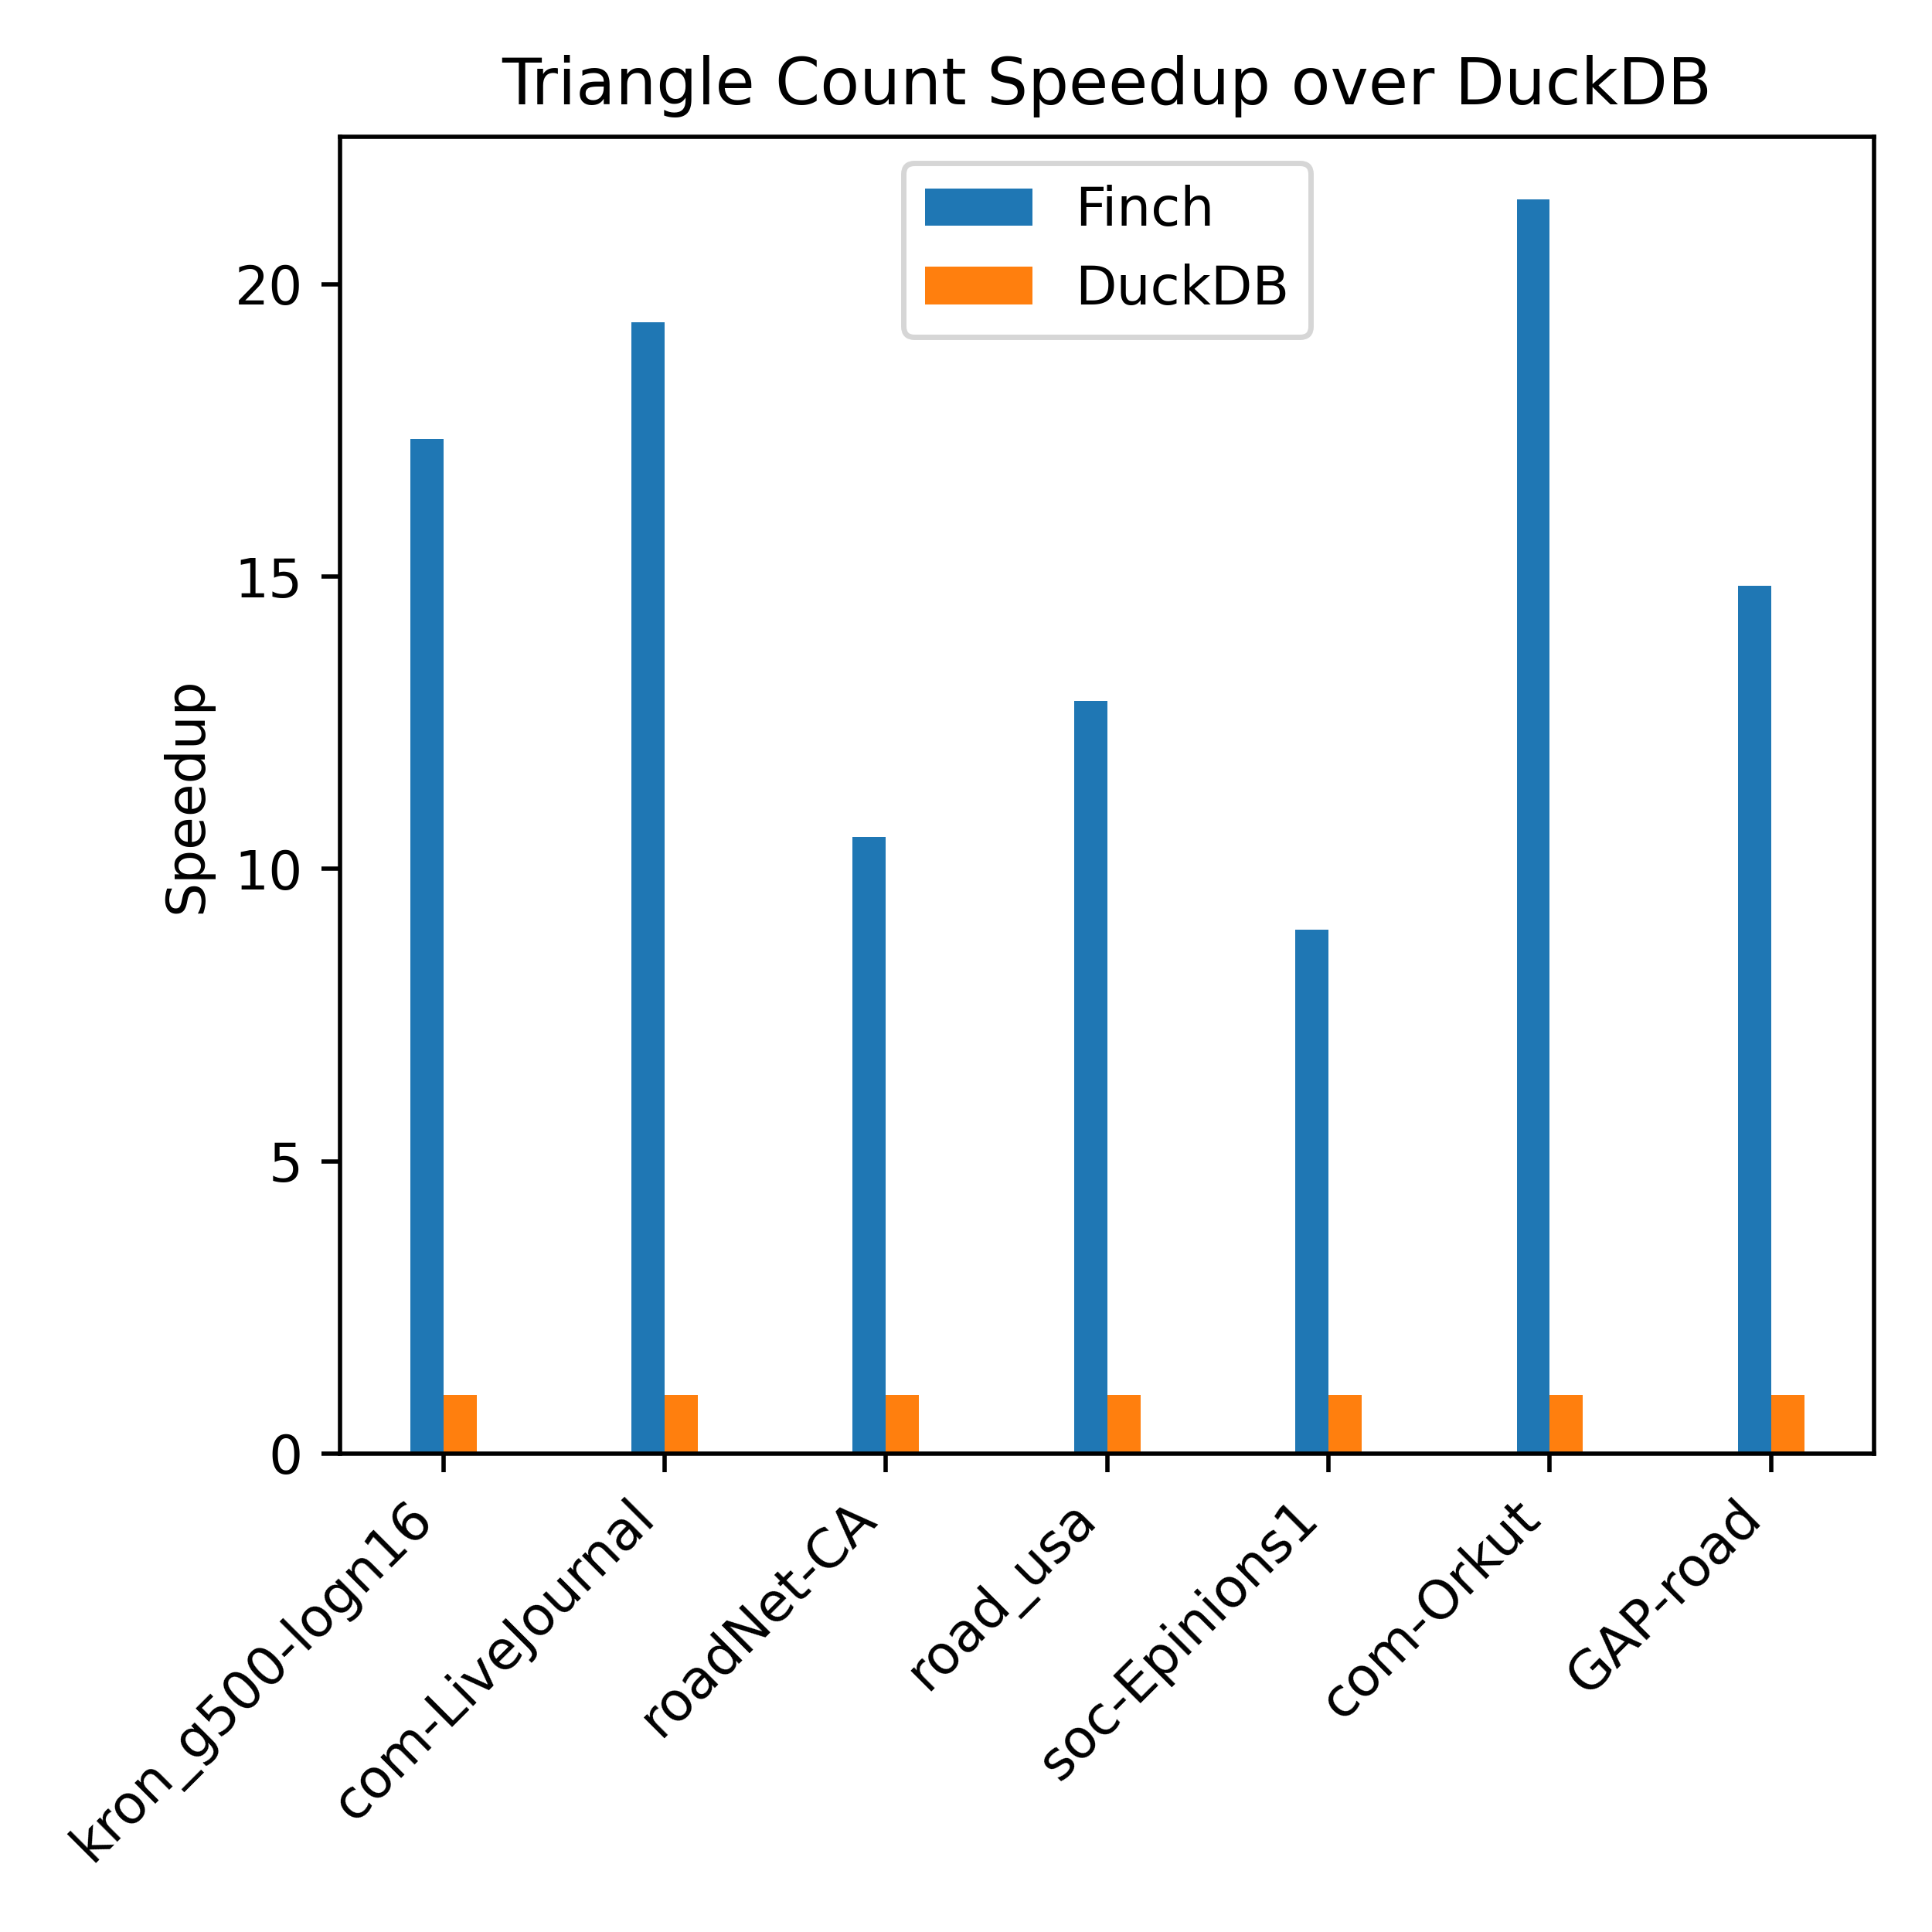
\includegraphics[width=140pt, height=135pt]{figures/triangle_count_speedup_over_duckdb.png} &
  \vspace{0pt} 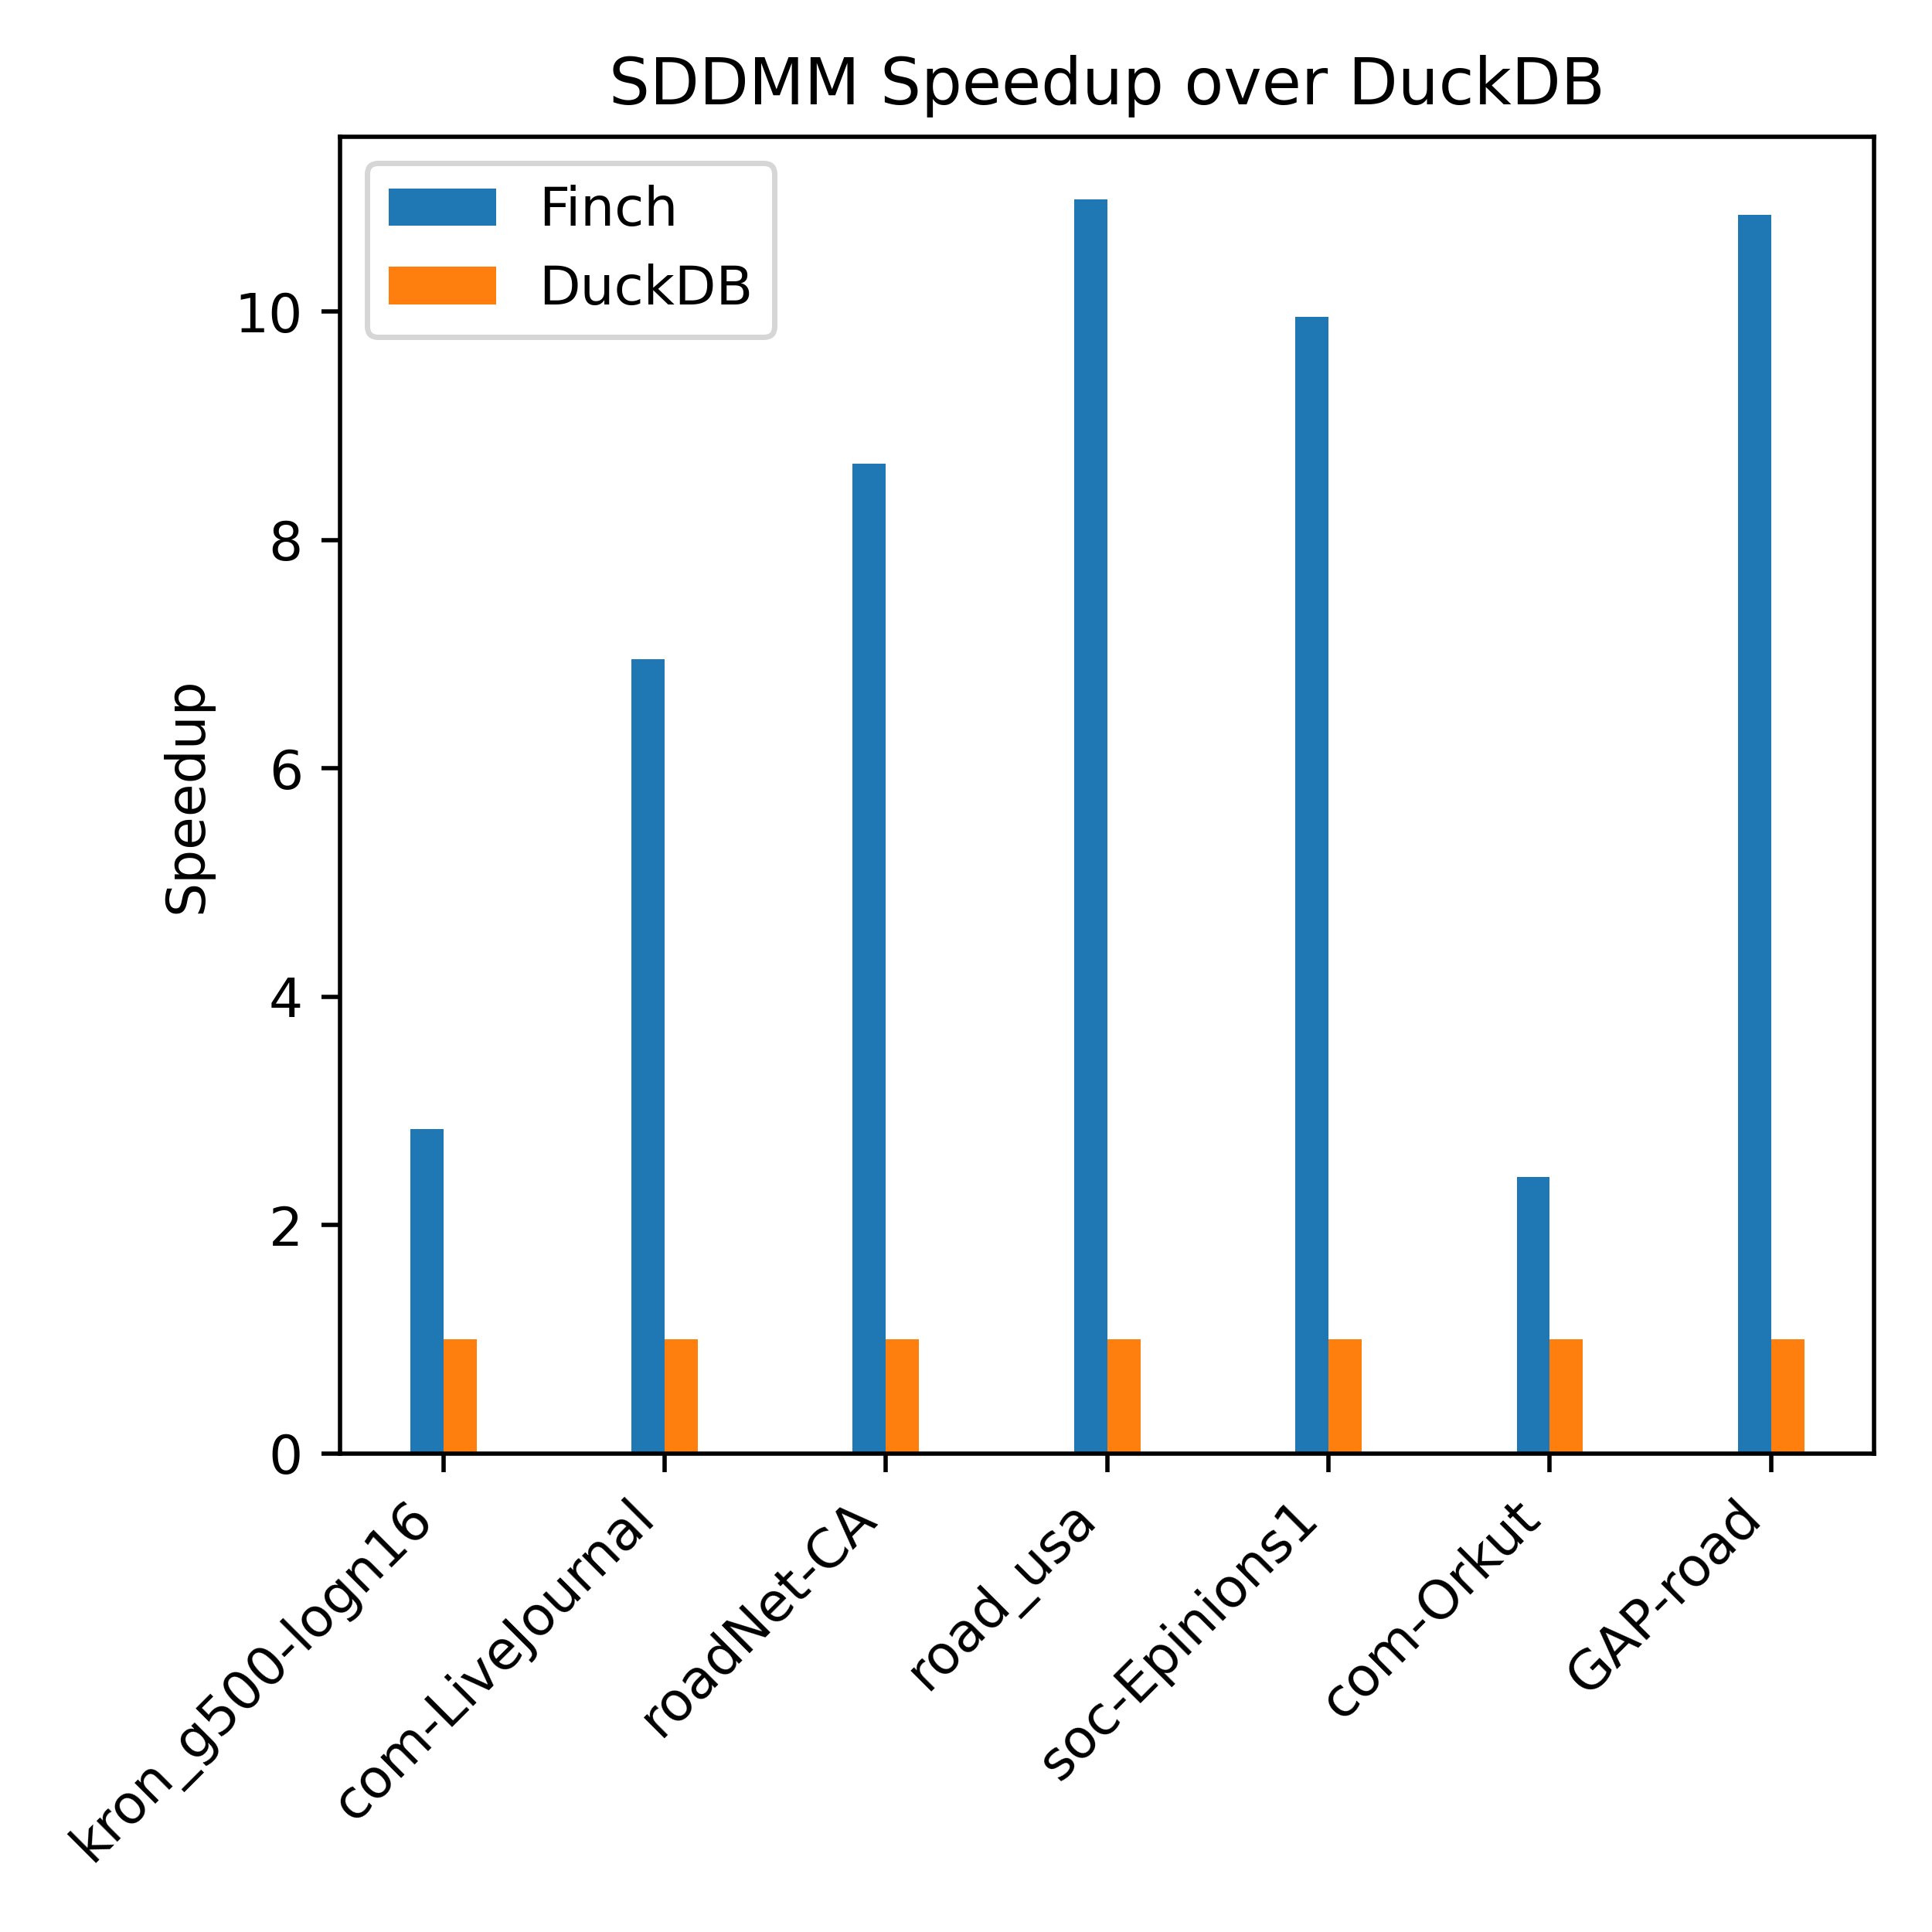
\includegraphics[width=140pt, height=135pt]{figures/sddmm_speedup_over_duckdb.png} &
  \vspace{0pt} 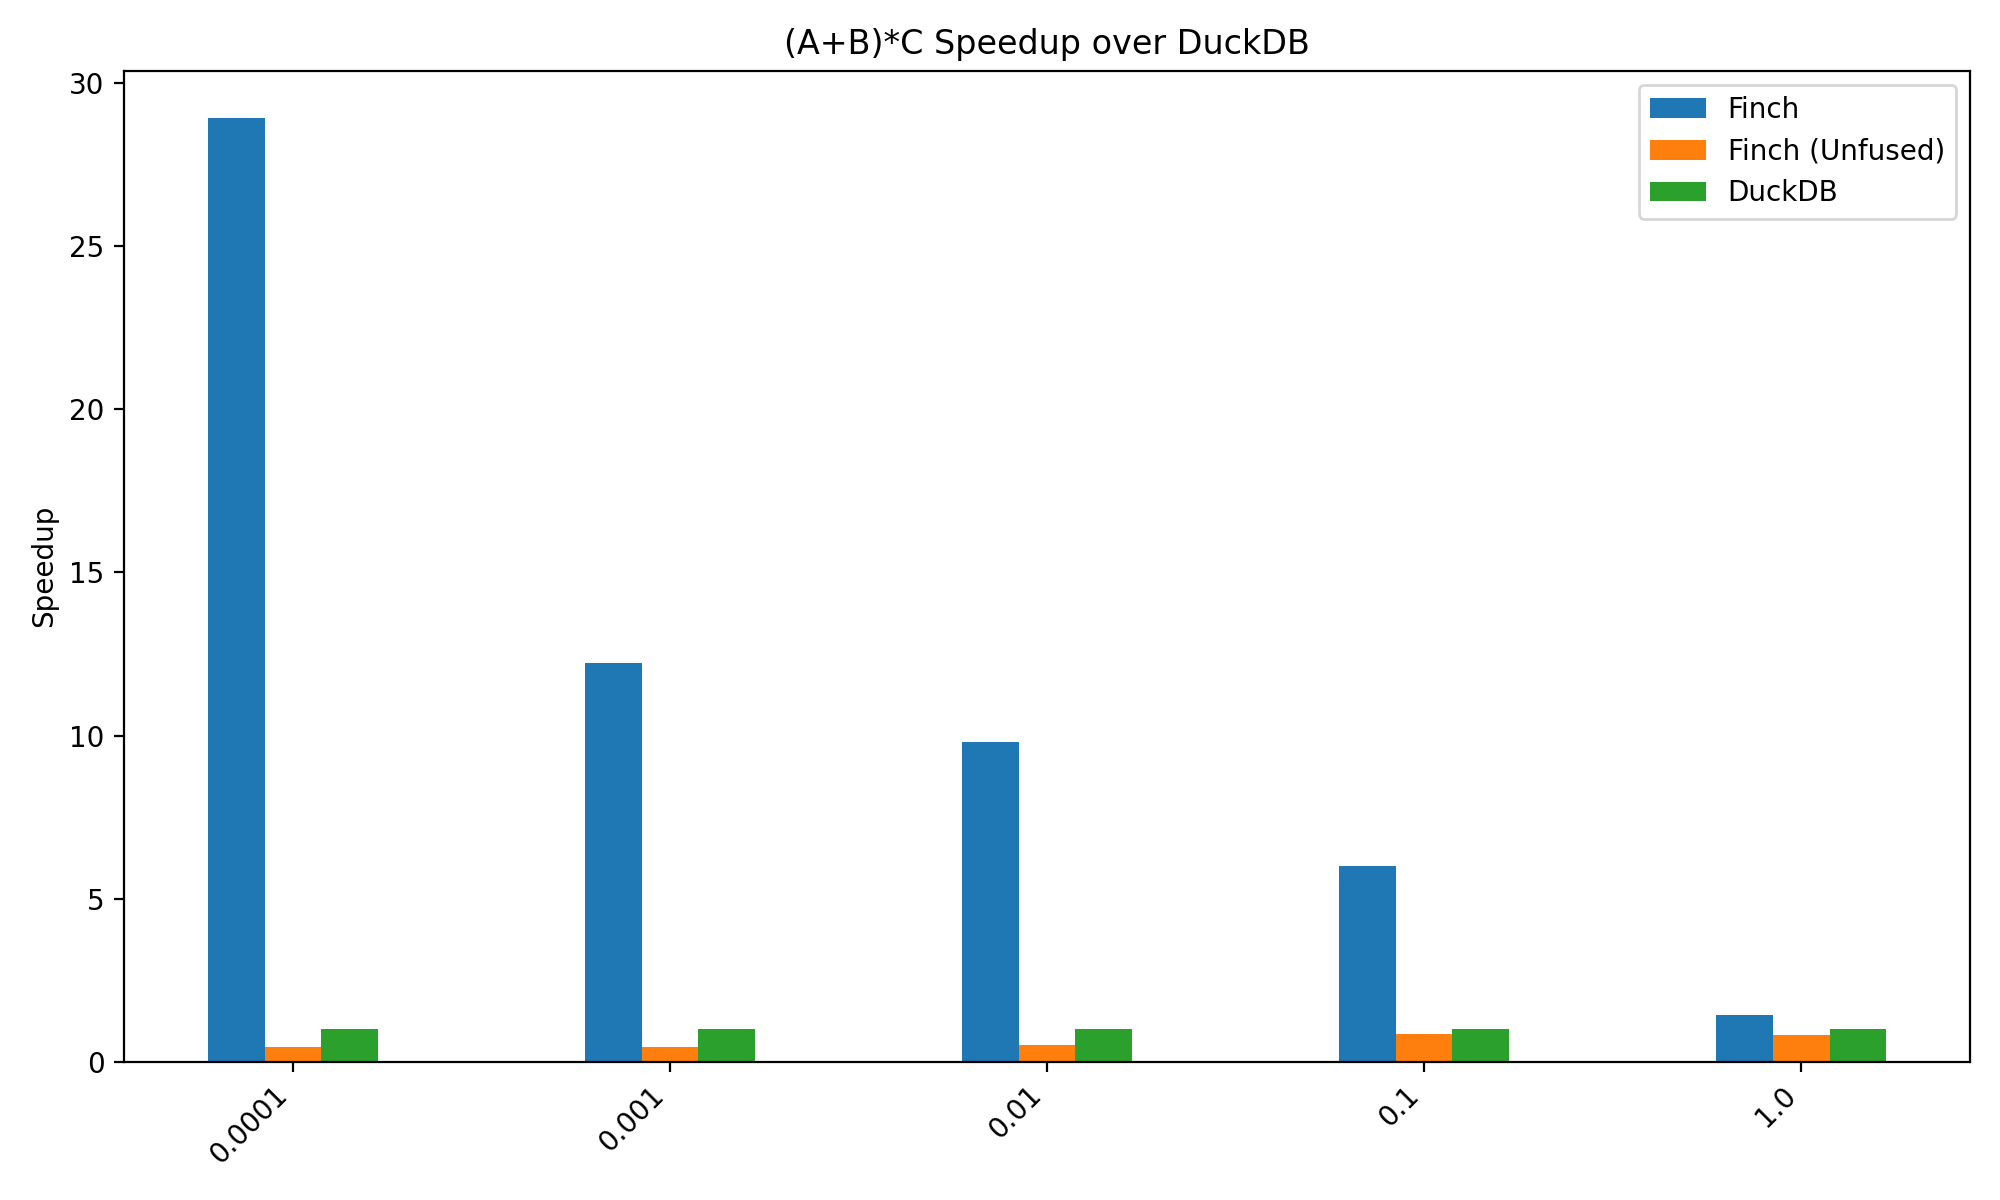
\includegraphics[width=140pt, height=123pt]{figures/elementwise_speedup_over_duckdb.png}
\end{tabular}
\caption{Performance of Finch Logic for common kernels.}
\end{figure}




%matmul, mttkrp, repeated ttm, triangle counting, multiple pointwise,
%in-place.
%dot((v^t .* u), w)) vs. 
%(v^t .* dot(u, w))

\willow{Note: I may want to explain format inference somewhere in here, but I'll
have to get to it a little later, perhaps after the paper deadline}
\willow{Note: I think it would be cool to include something about how we support
numerically stable norms and argmin in this model}